\documentclass{article}
%\documentstyle[11pt,handout,psfig]{article}

\usepackage{fullpage,amssymb,amsmath,epsf}
\usepackage[12pt]{extsizes}

%These give really tight margins:
%\setlength{\topmargin}{-0.3in}
%\setlength{\textheight}{8.10in}
%\setlength{\textwidth}{5.8in}
%\setlength{\baselineskip}{0.1875in}
%\addtolength{\leftmargin}{-2.775in}
%\setlength{\footskip}{0.45in}
%\setlength{\oddsidemargin}{0.5in}
%\setlength{\evensidemargin}{0.5in}
%%\setlength{\headsep}{0pt}
%%\setlength{\headheight}{0pt}

%\setlength{\topmargin}{-0.5in}
\setlength{\textheight}{8in}
%\setlength{\textwidth}{5.0in}
%\setlength{\baselineskip}{0.1875in}
%\addtolength{\leftmargin}{-2.775in}
%\setlength{\footskip}{0.45in}
%\setlength{\oddsidemargin}{0.5in}
%\setlength{\evensidemargin}{0.5in}
%%\setlength{\headsep}{0pt}
%%\setlength{\headheight}{0pt}


\markright{XCS229i}
\pagestyle{myheadings}

\newcommand{\newsec}{\section}
\newcommand{\denselist}{\itemsep 0pt\partopsep 0pt}
\newcommand{\bitem}{\begin{itemize}\denselist}
\newcommand{\eitem}{\end{itemize}}
\newcommand{\benum}{\begin{enumerate}\denselist}
\newcommand{\eenum}{\end{enumerate}}

\newcommand{\fig}[1]{\private{\begin{center}
{\Large\bf ({#1})}
\end{center}}}

\newcommand{\cpsf}[1]{{\centerline{\psfig{#1}}}}
\newcommand{\mytitle}[1]{\centerline{\LARGE\bf #1}}

\newcommand{\myw}{{\bf w}}

\newcommand{\mypar}[1]{\vspace{1ex}\noindent{\bf {#1}}}

\def\thmcolon{\hspace{-.85em} {\bf :} }

\newtheorem{THEOREM}{Theorem}[section]
\newenvironment{theorem}{\begin{THEOREM} \thmcolon }%
                        {\end{THEOREM}}
\newtheorem{LEMMA}[THEOREM]{Lemma}
\newenvironment{lemma}{\begin{LEMMA} \thmcolon }%
                      {\end{LEMMA}}
\newtheorem{COROLLARY}[THEOREM]{Corollary}
\newenvironment{corollary}{\begin{COROLLARY} \thmcolon }%
                          {\end{COROLLARY}}
\newtheorem{PROPOSITION}[THEOREM]{Proposition}
\newenvironment{proposition}{\begin{PROPOSITION} \thmcolon }%
                            {\end{PROPOSITION}}
\newtheorem{DEFINITION}[THEOREM]{Definition}
\newenvironment{definition}{\begin{DEFINITION} \thmcolon \rm}%
                            {\end{DEFINITION}}
\newtheorem{CLAIM}[THEOREM]{Claim}
\newenvironment{claim}{\begin{CLAIM} \thmcolon \rm}%
                            {\end{CLAIM}}
\newtheorem{EXAMPLE}[THEOREM]{Example}
\newenvironment{example}{\begin{EXAMPLE} \thmcolon \rm}%
                            {\end{EXAMPLE}}
\newtheorem{REMARK}[THEOREM]{Remark}
\newenvironment{remark}{\begin{REMARK} \thmcolon \rm}%
                            {\end{REMARK}}
%\newenvironment{proof}{\noindent {\bf Proof:} \hspace{.677e\nexp}}%
%                      {}

%theorem
\newcommand{\thm}{\begin{theore\nexp}}
%lemma
\newcommand{\lem}{\begin{lemma}}
%proposition
\newcommand{\pro}{\begin{propositio\di}}
%definition
\newcommand{\dfn}{\begin{definitio\di}}
%remark
\newcommand{\rem}{\begin{remark}}
%example
\newcommand{\xam}{\begin{example}}
%corollary
\newcommand{\cor}{\begin{corollary}}
%proof
\newcommand{\prf}{\noindent{\bf Proof:} }
%end theorem
\newcommand{\ethm}{\end{theore\nexp}}
%end lemma
\newcommand{\elem}{\end{lemma}}
%end proposition
\newcommand{\epro}{\end{propositio\di}}
%end definition
\newcommand{\edfn}{\bbox\end{definitio\di}}
%end remark
\newcommand{\erem}{\bbox\end{remark}}
%end example
\newcommand{\exam}{\bbox\end{example}}
%end corollary
\newcommand{\ecor}{\end{corollary}}
%end proof
\newcommand{\eprf}{\bbox\vspace{0.1i\di}}
%begin equation
\newcommand{\beqn}{\begin{equatio\di}}
%end equation
\newcommand{\eeqn}{\end{equatio\di}}

%\newcommand{\eqref}[1]{Eq.~\ref{#1}}

\newcommand{\KB}{\mbox{\it KB\/}}
\newcommand{\infers}{\vdash}
\newcommand{\sat}{\models}
\newcommand{\bbox}{\vrule height7pt width4pt depth1pt}

\newcommand{\act}[1]{\stackrel{{#1}}{\rightarrow}}
\newcommand{\at}[1]{^{(#1)}}

\newcommand{\argmax}{{\rm argmax}}

\newcommand{\rimp}{\Rightarrow}
\newcommand{\dimp}{\Leftrightarrow}

\newcommand{\bX}{\mbox{\boldmath $X$}}
\newcommand{\bY}{\mbox{\boldmath $Y$}}
\newcommand{\bZ}{\mbox{\boldmath $Z$}}
\newcommand{\bU}{\mbox{\boldmath $U$}}
\newcommand{\bE}{\mbox{\boldmath $E$}}
\newcommand{\bx}{\mbox{\boldmath $x$}}
\newcommand{\be}{\mbox{\boldmath $e$}}
\newcommand{\by}{\mbox{\boldmath $y$}}
\newcommand{\bz}{\mbox{\boldmath $z$}}
\newcommand{\bu}{\mbox{\boldmath $u$}}
\newcommand{\bd}{\mbox{\boldmath $d$}}
\newcommand{\smbx}{\mbox{\boldmath $\scriptstyle x$}}
\newcommand{\smbd}{\mbox{\boldmath $\scriptstyle d$}}
\newcommand{\smby}{\mbox{\boldmath $\scriptstyle y$}}
\newcommand{\smbe}{\mbox{\boldmath $\scriptstyle e$}}

\newcommand{\Parents}{\mbox{\it Parents\/}}
\newcommand{\B}{{\cal B}}
\newcommand{\calH}{{\cal H}}

\newcommand{\word}[1]{\mbox{\it #1\/}}
\newcommand{\Action}{\word{Actio\di}}
\newcommand{\Proposition}{\word{Propositio\di}}
\newcommand{\true}{\word{true}}
\newcommand{\false}{\word{false}}
\newcommand{\Pre}{\word{Pre}}
\newcommand{\Add}{\word{Add}}
\newcommand{\Del}{\word{Del}}
\newcommand{\Result}{\word{Result}}
\newcommand{\Regress}{\word{Regress}}
\newcommand{\Maintain}{\word{Maintai\di}}

\newcommand{\bor}{\bigvee}
\newcommand{\invert}[1]{{#1}^{-1}}

\newcommand{\commentout}[1]{}

\newcommand{\bmu}{\mbox{\boldmath $\mu$}}
\newcommand{\btheta}{\mbox{\boldmath $\theta$}}
\newcommand{\IR}{\mbox{$I\!\!R$}}

\newcommand{\tval}[1]{{#1}^{1}}
\newcommand{\fval}[1]{{#1}^{0}}

\newcommand{\tr}{{\rm tr}}
\newcommand{\vecy}{{\vec{y}}}
\renewcommand{\Re}{{\mathbb R}}

\def\twofigbox#1#2{%
\noindent\begin{minipage}{\textwidth}%
\epsfxsize=0.35\maxfigwidth
\noindent \epsffile{#1}\hfill
\epsfxsize=0.35\maxfigwidth
\epsffile{#2}\\
\makebox[0.35\textwidth]{(a)}\hfill\makebox[0.35\textwidth]{(b)}%
\end{minipage}}

\def\twofigboxcd#1#2{%
\noindent\begin{minipage}{\textwidth}%
\epsfxsize=0.35\maxfigwidth
\noindent \epsffile{#1}\hfill
\epsfxsize=0.35\maxfigwidth
\epsffile{#2}\\
\makebox[0.35\textwidth]{(c)}\hfill\makebox[0.35\textwidth]{(d)}%
\end{minipage}}

\def\twofigboxnolabel#1#2{%
\begin{minipage}{\textwidth}%
\epsfxsize=0.35\maxfigwidth
\noindent \epsffile{#1}\hfill
\epsfxsize=0.35\maxfigwidth
\epsffile{#2}\\
%\makebox[0.48\textwidth]{(a)}\hfill\makebox[0.48\textwidth]{(b)}%
\end{minipage}
}

\def\twofigboxnolabelFive#1#2{%
\begin{minipage}{\textwidth}%
\hbox to 0.5in{}\epsfxsize=0.35\maxfigwidth
\noindent \epsffile{#1}\hfill
\epsfxsize=0.35\maxfigwidth
\epsffile{#2}\hbox to 0.5in{}\\
%\makebox[0.48\textwidth]{(a)}\hfill\makebox[0.48\textwidth]{(b)}%
\end{minipage}
}

\def\threefigbox#1#2#3{%
\noindent\begin{minipage}{\textwidth}%
\epsfxsize=0.33\maxfigwidth
\noindent \epsffile{#1}\hfill
\epsfxsize=0.33\maxfigwidth
\noindent \epsffile{#2}\hfill 
\epsfxsize=0.33\maxfigwidth
\epsffile{#3}\\
\makebox[0.31\textwidth]{{\scriptsize (a)}}\hfill%
\makebox[0.31\textwidth]{{\scriptsize (b)}}\hfill
\makebox[0.31\textwidth]{{\scriptsize (c)}}%
\smallskip
\end{minipage}}

\def\threefigboxnolabel#1#2#3{%
\noindent\begin{minipage}{\textwidth}%
\epsfxsize=0.33\maxfigwidth
\noindent \epsffile{#1}\hfill
\epsfxsize=0.33\maxfigwidth
\noindent \epsffile{#2}\hfill 
\epsfxsize=0.33\maxfigwidth
\epsffile{#3}\\
%\makebox[0.31\textwidth]{{\scriptsize (a)}}\hfill%
%\makebox[0.31\textwidth]{{\scriptsize (b)}}\hfill
%\makebox[0.31\textwidth]{{\scriptsize (c)}}%
%\smallskip
\end{minipage}}

\newlength{\maxfigwidth}
\setlength{\maxfigwidth}{\textwidth}
%\def\captionsize {\footnotesize}
\def\captionsize {}

\newcommand{\xsi}{{x^{(i)}}}
\newcommand{\xsd}{{x^{(d)}}}
\newcommand{\xsj}{{x^{(j)}}}
\newcommand{\ysi}{{y^{(i)}}}
\newcommand{\ysj}{{y^{(j)}}}
\newcommand{\gsi}{{\gamma^{(i)}}}
\newcommand{\wsi}{{w^{(i)}}}
\newcommand{\esi}{{\epsilon^{(i)}}}
\newcommand{\calN}{{\cal N}}
\newcommand{\calX}{{\cal X}}
\newcommand{\calY}{{\cal Y}}
\newcommand{\calL}{{\cal L}}
\newcommand{\calP}{{\cal P}}
\newcommand{\calD}{{\cal D}}
\newcommand{\ytil}{{\tilde{y}}}

\newcommand{\Ber}{{\rm Bernoulli}}
\newcommand{\E}{{\rm E}}

\newcommand{\pstar}{{p^{\ast}}}
\newcommand{\bstar}{{b^{\ast}}}
\newcommand{\dstar}{{d^{\ast}}}
\newcommand{\wstar}{{w^{\ast}}}
\newcommand{\alphastar}{\alpha^{\ast}}
\newcommand{\alphastari}{{\alpha_i^{\ast}}}
\newcommand{\betastar}{{\beta^{\ast}}}
\newcommand{\tol}{{\textit tol}}
\newcommand{\phihat}{\hat\phi}
\newcommand{\ehat}{\hat\varepsilon}
\newcommand{\hhat}{\hat{h}}
\newcommand{\hstar}{h^\ast}
\newcommand{\VC}{{\rm VC}}

\newcommand{\hwb}{{h_{w,b}}}

\usepackage{graphicx}

%\renewcommand{\epsffile}[1]{
%	\includegraphics[width=\epsfxsize]{#1}
%}

\newcommand{\di}{{d}}
\newcommand{\nexp}{{n}}
\newcommand{\vcd}{{\textbf{D}}}

\begin{document}
\title{XCS229i Lecture Notes}
\author{Andrew Ng}
%\date{Lectures from 1/7/03 to 1/16/03}
% \date{slightly updated by TM on \today}
\date{}
\maketitle


\section*{Supervised learning}


Let's start by talking about a few examples of supervised learning problems.
Suppose we have a dataset giving the living areas and prices of 47 houses from
Portland, Oregon:
%\footnote{This data was obtained from public postings on Craigslist and can be downloaded from the course web page.
% % (2007 data)
%Source: {\tt http://portland.craigslist.org/rfs/}.}
%
% Data collected by Dan Ramage.
\begin{center}
\begin{tabular}{c|c}
Living area (feet$^2$) & Price (1000\$s) \\ \hline
2104 & 400  \\
1600 & 330  \\
2400 & 369  \\
1416 & 232  \\
3000 & 540  \\
\vdots & \vdots
\end{tabular}
\end{center}

We can plot this data:
\begin{center}
% Commenting out since outdated class eps to integrate images
% \epsfxsize=3in
% \epsffile{housingData.eps}
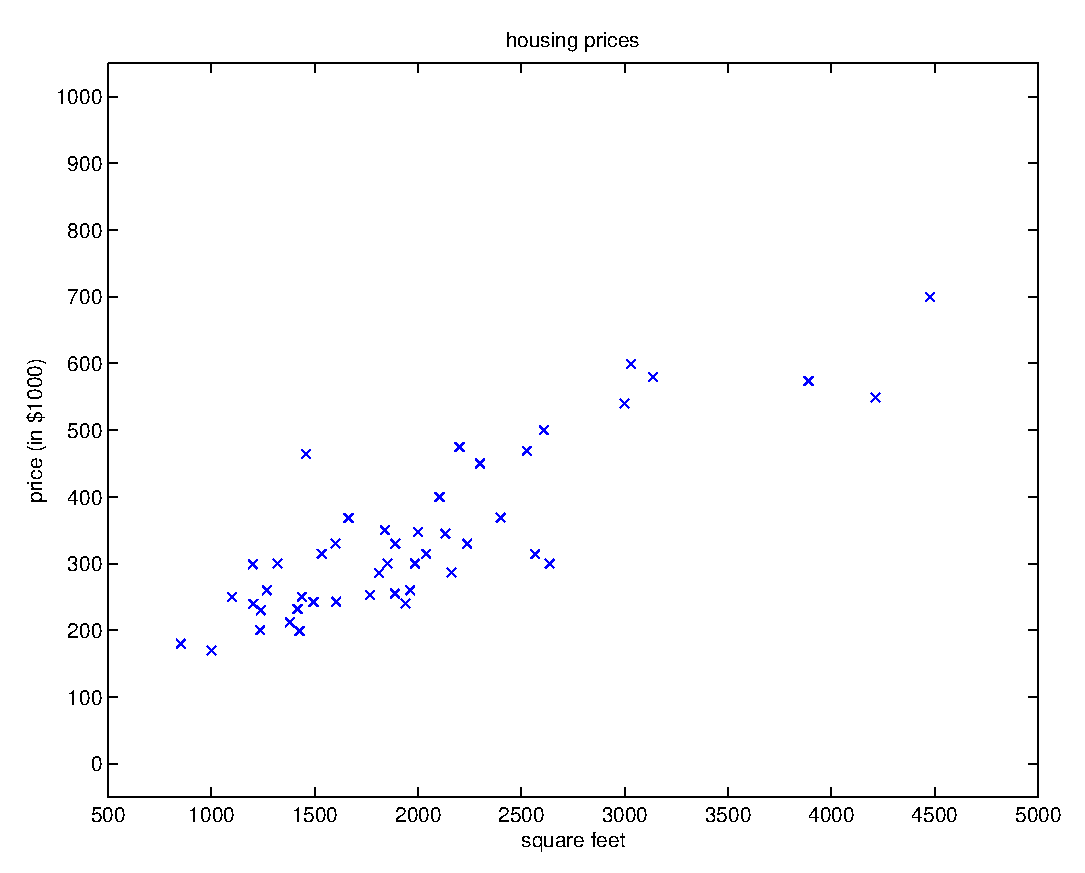
\includegraphics[scale=0.4]{housingData.eps}
\end{center}

Given data like this, how can we learn to predict the prices of other houses in Portland, as a function
of the size of their living areas?

To establish notation for future use, we'll use $x^{(i)}$ to denote the ``input'' variables (living area in this example), also called
input {\bf features}, and $y^{(i)}$ to denote the ``output'' or {\bf target}
variable that we are trying to predict (price).  A pair $(\xsi, \ysi)$ is called
a {\bf training example}, and the dataset that we'll be using to learn---a list of $\nexp$ training
examples $\{(\xsi,\ysi); i=1,\ldots,\nexp\}$---is called a {\bf training set}.  Note that the superscript
``${(i)}$'' in the notation is simply an index into the training set, and has nothing
to do with exponentiation.  We will also use $\calX$ denote the space of input
values, and $\calY$ the space of output values.  In this example,
$\calX = \calY = \Re$.

To describe the supervised learning problem slightly more formally,
our goal is, given a training set, to learn a function
$h : \calX \mapsto \calY$ so that $h(x)$ is a ``good'' predictor
for the corresponding value of $y$.  For historical reasons, this
function $h$ is called a {\bf hypothesis}.  Seen pictorially, the
process is therefore
like this:

\begin{center}
% Commenting out since outdated class eps to integrate images
% \epsfxsize=2in
% \epsffile{learningProcess.eps}
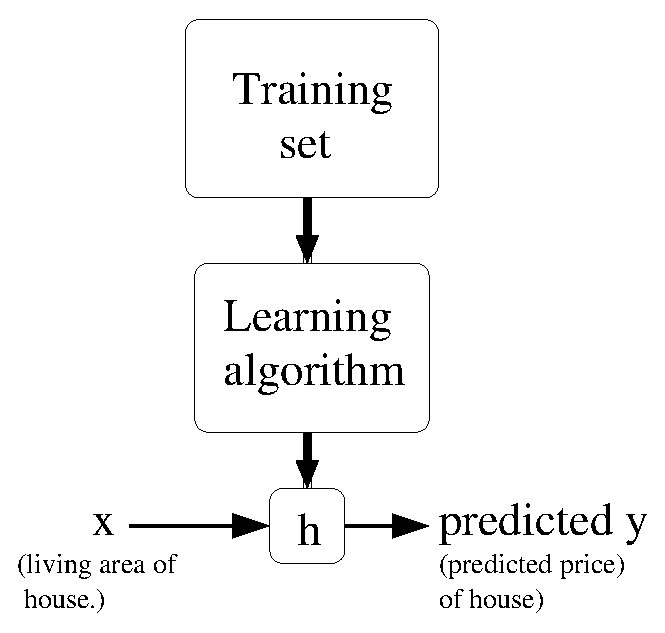
\includegraphics[scale=0.4]{learningProcess.eps}
\end{center}

When the target variable that we're trying to predict is continuous, such as in our housing
example, we call the learning problem a {\bf regression} problem.  When $y$ can take
on only a small number of discrete values (such as if, given the living area,
we wanted to predict if a dwelling is a house or an apartment, say), we call
it a {\bf classification} problem.

\newpage
\part{Linear Regression}

To make our housing example more interesting, let's consider a slightly richer
dataset in which we also know the number of bedrooms in each house:

\begin{center}
\begin{tabular}{c|c|c}
Living area (feet$^2$) & \#bedrooms & Price (1000\$s) \\ \hline
2104 & 3 & 400  \\
1600 & 3 & 330  \\
2400 & 3 & 369  \\
1416 & 2 & 232  \\
3000 & 4 & 540  \\
\vdots & \vdots  & \vdots
\end{tabular}
\end{center}

Here, the $x$'s are two-dimensional vectors in $\Re^2$.  For instance,
$x^{(i)}_1$ is the living area of the $i$-th house in the training set, and
$x^{(i)}_2$ is its number of bedrooms.  (In general, when designing a learning
problem, it will be up to you to decide what features to choose, so if you
are out in Portland gathering housing data, you might also decide to include
other features such as whether each house has a fireplace, the number of
bathrooms, and so on.  We'll say more about feature selection later, but
for now let's take the features as given.)

To perform supervised learning, we must decide how we're going to
represent functions/hypotheses $h$ in a computer.  As an initial choice,
let's say we decide to approximate $y$ as a linear function of $x$:
\[
h_\theta(x) = \theta_0 + \theta_1 x_1 + \theta_2 x_2
\]
Here, the $\theta_i$'s are the {\bf parameters} (also called {\bf weights})
parameterizing the space
of linear functions mapping from $\calX$ to $\calY$.  When there is no
risk of confusion, we will drop the $\theta$ subscript in $h_\theta(x)$,
and write it more simply as $h(x)$.  To simplify our notation, we also
introduce the convention of letting $x_0 = 1$ (this is the
{\bf intercept term}), so that
\[
h(x) = \sum_{i=0}^\di \theta_i x_i = \theta^T x,
\]
where on the right-hand side above we are viewing $\theta$ and $x$ both as vectors, and
here $\di$ is the number of input variables (not counting $x_0$).

Now, given a training set, how do we pick, or learn, the parameters $\theta$?
One reasonable method seems to be to make $h(x)$ close to $y$, at least
for the training examples we have.  To formalize this, we will define a
function that measures, for each value of the $\theta$'s, how close
the $h(\xsi)$'s are to the corresponding $\ysi$'s.  We define the {\bf cost function}:
\[
J(\theta) = \frac{1}{2} \sum_{i=1}^{\nexp} (h_\theta(\xsi) - \ysi)^2.
\]
If you've seen linear regression before, you may recognize this as the
familiar least-squares cost function that gives rise to the
{\bf ordinary least squares} regression model.  Whether or not you have
seen it previously, let's keep going, and we'll eventually show this to
be a special case of a much broader family of algorithms.

%Later, we will derive
%a fascinating result in which we show this model to be a special case
%of a much broader family of algorithms.


\section{LMS algorithm}

We want to choose $\theta$ so as to minimize $J(\theta)$.  To do so, let's use a
search algorithm that starts with some ``initial guess'' for $\theta$, and that
repeatedly changes $\theta$ to make $J(\theta)$ smaller, until hopefully we converge
to a value of $\theta$ that minimizes $J(\theta)$.  Specifically, let's
consider the {\bf gradient descent} algorithm, which starts with some
initial $\theta$, and repeatedly performs the update:
\[
\theta_j := \theta_j - \alpha \frac{\partial}{\partial \theta_j} J(\theta).
\]
(This update is simultaneously performed for all values of $j=0,\ldots,\di$.)
Here, $\alpha$ is called the {\bf learning rate}.  This is a very natural
algorithm that repeatedly takes a step in the direction of steepest
decrease of $J$.

In order to implement this algorithm, we have to work out what is the partial
derivative term on the right hand side.  Let's first work it out for the
case of if we have only one training example $(x,y)$, so that we can neglect
the sum in the definition of $J$.  We have:
\begin{eqnarray*}
\frac{\partial}{\partial \theta_j} J(\theta) &=&
\frac{\partial}{\partial \theta_j} \frac{1}{2} \left(h_\theta(x) - y\right)^2 \\
&=& 2 \cdot \frac{1}{2} \left(h_\theta(x) - y\right) \cdot
\frac{\partial}{\partial \theta_j} (h_\theta(x) - y) \\
%&=& \left(h_\theta(x) - y\right) \cdot
%\frac{\partial}{\partial \theta_j} h_\theta(x) - y \\
&=& \left(h_\theta(x) - y\right) \cdot
\frac{\partial}{\partial \theta_j} \left( \sum_{i=0}^\di \theta_i x_i - y \right)\\
&=& \left(h_\theta(x) - y\right) x_j
\end{eqnarray*}

For a single training example, this gives the update rule:\footnote{We use the
notation ``$a := b$'' to denote an operation (in a computer program) in
which we \emph{set} the value of a variable $a$ to be equal to the value of $b$.  In other
words, this operation overwrites $a$ with the value of $b$.  In contrast, we will
write ``$a = b$'' when we are asserting a statement of fact, that the value of $a$ is
equal to the value of $b$.}
\[
\theta_j := \theta_j + \alpha \left(\ysi - h_\theta(\xsi)\right) x^{(i)}_j.  %\label{eqn-lms}
\]
The rule is called the {\bf LMS} update rule (LMS stands for ``least mean squares''),
and is also known as the {\bf Widrow-Hoff} learning rule.
This rule has several properties that seem natural and intuitive. For instance, the
magnitude of the update is proportional to
the {\bf error} term
$(\ysi - h_\theta(\xsi))$; thus, for instance, if we are encountering a training
example on which our prediction nearly matches the actual value of $\ysi$,
then we find that there is little need to change the parameters; in contrast,
a larger change to the parameters will be made if our prediction
$h_\theta(\xsi)$ has a large error (i.e., if it is very far from $\ysi$).

We'd derived the LMS rule for when there was only a single training example.  There are two
ways to modify this method for a training set of more than one example.  The first is
replace it with the following algorithm:
\begin{enumerate}
\item[] Repeat until convergence $\{$
\begin{enumerate}
\item[]\begin{align}\theta_j := \theta_j + \alpha \sum_{i=1}^\nexp \left(\ysi - h_\theta(\xsi)\right) x^{(i)}_j, \textup{(for every $j$)}\label{eqn:gd}\end{align}
\end{enumerate}
\item[] $\}$
\end{enumerate}

By grouping the updates of the coordinates into an update of the vector $\theta$, we can rewrite update~\eqref{eqn:gd} in a slightly more succinct way:
\begin{align}
\theta := \theta + \alpha \sum_{i=1}^\nexp \left(\ysi - h_\theta(\xsi)\right) x^{(i)} \nonumber
\end{align}

The reader can easily verify that the quantity in the summation in the update rule above
is just
$\partial J(\theta)/\partial\theta_j$ (for the original definition of $J$).  So,
this is simply gradient descent on the original cost function $J$.  This method
looks at every example in the entire training set on every step, and is
called {\bf batch gradient descent}.  Note that, while gradient descent can
be susceptible to local minima in general, the optimization problem we have
posed here for linear regression has only one global, and no other local, optima; thus
gradient descent always converges (assuming the learning rate $\alpha$ is not too large)
to the global minimum.  Indeed, $J$ is a convex quadratic function.  Here is an
example of gradient descent as it is run to minimize a quadratic function.
\begin{center}
% Commenting out since outdated class eps to integrate images
% \epsfxsize=3in
% \epsffile{quadracticGD20.eps}
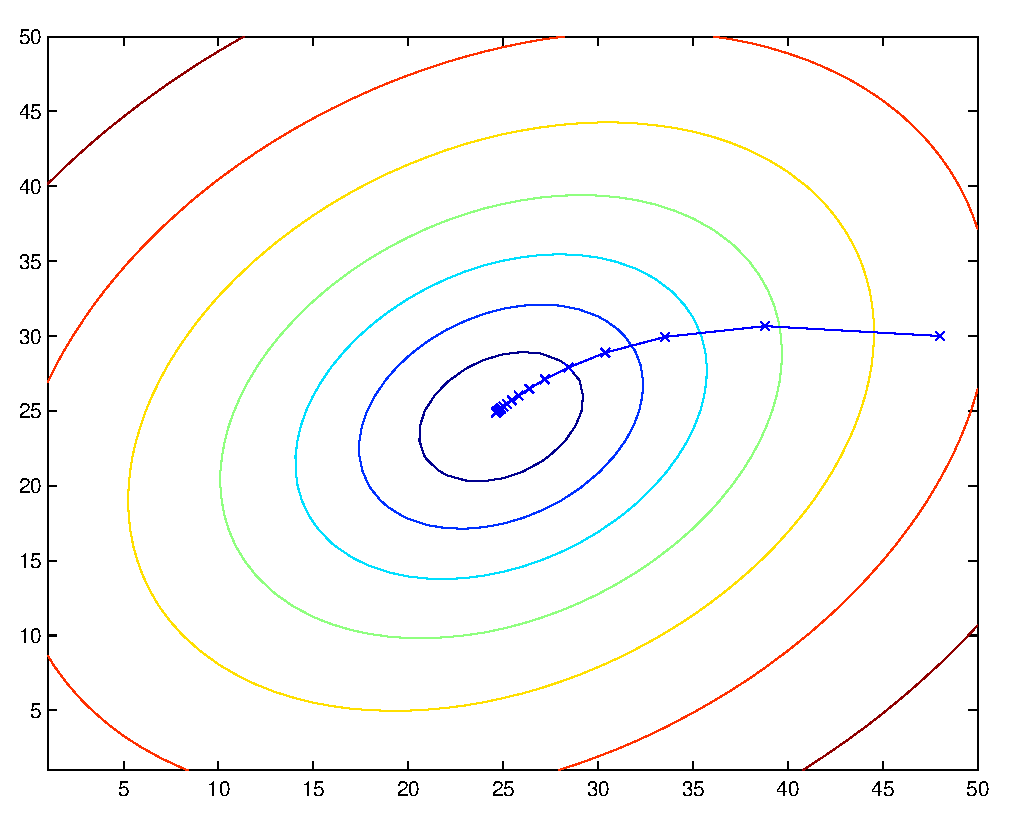
\includegraphics[scale=0.4]{quadracticGD20.eps}
\end{center}
The ellipses shown above are the contours of a quadratic function.  Also
shown is the trajectory taken by gradient descent, which was initialized
at (48,30).  The $x$'s in the figure (joined by straight lines) mark the
successive values of $\theta$ that gradient descent went through.

When we run batch gradient descent to fit $\theta$ on our previous dataset,
to learn to predict housing price as a function of living area, we
obtain $\theta_0 = 71.27$, $\theta_1 = 0.1345$.  If we plot
$h_\theta(x)$ as a function of $x$ (area), along with the training data, we
obtain the
following figure:
\begin{center}
% Commenting out since outdated class eps to integrate images
% \epsfxsize=3in
% \epsffile{housingGDConverged.eps}
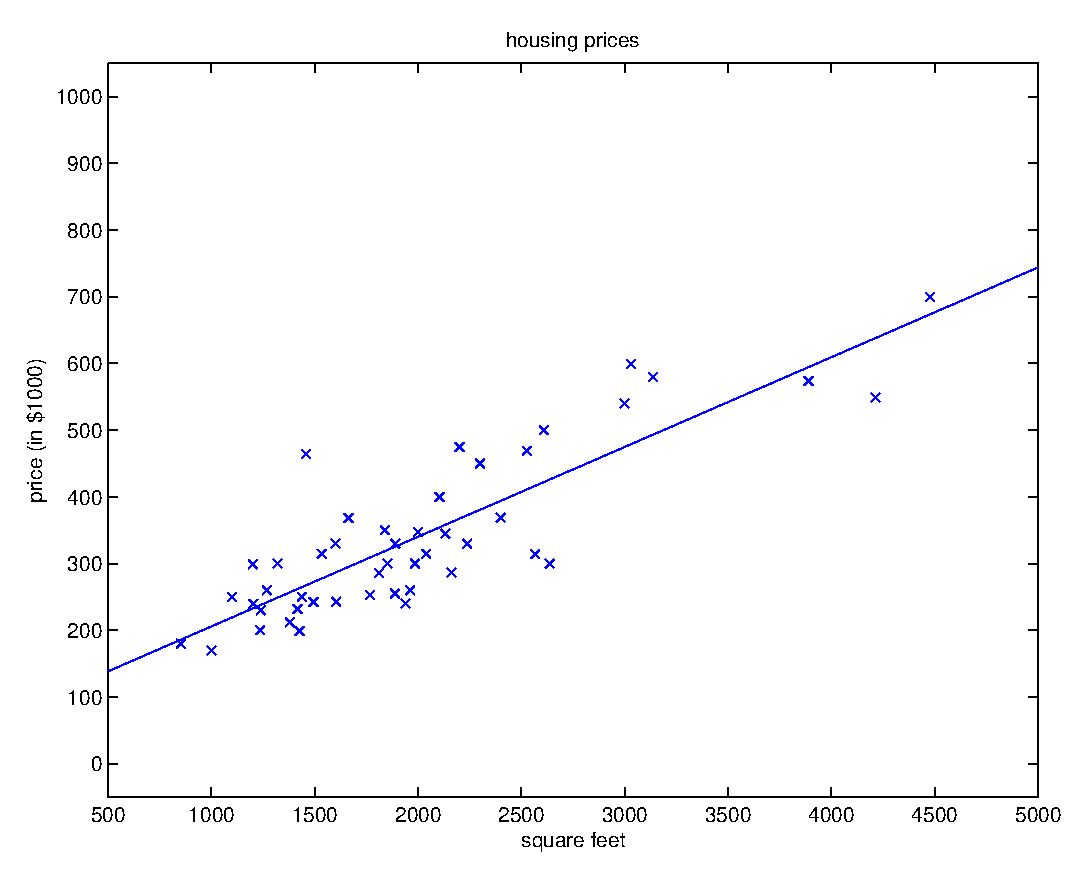
\includegraphics[scale=0.5]{housingGDConverged.eps}
\end{center}
If the number of bedrooms were included as one of the input features as well,
we get $\theta_0 = 89.60, \theta_1 = 0.1392$, $\theta_2 = -8.738$.

The above results were obtained with batch gradient descent.  There is an
alternative to batch gradient descent that also works very well.
Consider the following algorithm:
\begin{enumerate}
\item[] Loop $\{$
\begin{enumerate}
\item[] for $i=1$ to $\nexp$, $\{$
\begin{enumerate}
\item[] \begin{align}\theta_j := \theta_j + \alpha \left(\ysi - h_\theta(\xsi)\right) x^{(i)}_j, ~~~(\textup{for every } j)\label{eqn:update}\end{align}
\end{enumerate}
\item[] $\}$
\end{enumerate}
\item[] $\}$
\end{enumerate}

By grouping the updates of the coordinates into an update of the vector $\theta$, we can rewrite update~\eqref{eqn:update} in a slightly more succinct way:
\begin{align}
\theta := \theta + \alpha \left(\ysi - h_\theta(\xsi)\right) x^{(i)} \nonumber
\end{align}

In this algorithm, we repeatedly run through the training set, and
each time we encounter a training example, we update the parameters
according to the gradient of the error with respect to that single training
example only.  This algorithm is called {\bf stochastic gradient descent}
(also {\bf incremental gradient descent}).
Whereas batch gradient descent has to scan through the entire training set
before taking a single step---a costly operation if $\nexp$ is large---stochastic
gradient descent can start making progress right away, and continues to make
progress with each example it looks at.  Often, stochastic gradient descent
gets $\theta$ ``close'' to the minimum much faster than batch
gradient descent.  (Note however that it may never ``converge'' to the minimum,
and the parameters $\theta$ will keep oscillating around the minimum
of $J(\theta)$; but in practice most of the values near the minimum will be
reasonably good approximations to the true minimum.\footnote{By slowly letting the learning rate $\alpha$
decrease to zero as the algorithm runs, it is also possible to ensure that
the parameters will converge to the global minimum rather than merely oscillate
around the minimum.})  For these reasons, particularly when the training
set is large, stochastic gradient descent is often preferred over batch
gradient descent.

\section{The normal equations}

Gradient descent gives one way of minimizing $J$.  Let's discuss a second
way of doing so, this time performing the minimization explicitly
and without resorting to an iterative algorithm.  In this method, we will
minimize $J$ by explicitly taking its derivatives with respect to the $\theta_j$'s,
and setting them to zero.  To enable us to do this without having to write reams
of algebra and pages full of matrices of derivatives, let's introduce some
notation for doing calculus with matrices.

\subsection{Matrix derivatives}

For a function $f : \Re^{\nexp\times \di} \mapsto \Re$ mapping from
$\nexp$-by-$\di$ matrices to the real numbers, we define the derivative
of $f$ with respect to $A$ to be:
\[
\nabla_A f(A) = \left[
\begin{tabular}{ccc}
$\frac{\partial f}{\partial A_{11}}$ & $\cdots$ & $\frac{\partial f}{\partial A_{1\di}}$  \\
$\vdots$ & $\ddots$ & $\vdots$ \\
$\frac{\partial f}{\partial A_{\nexp1}}$ & $\cdots$ & $\frac{\partial f}{\partial A_{\nexp\di}}$
\end{tabular}
\right]
\]
Thus, the gradient $\nabla_A f(A)$ is itself an $\nexp$-by-$\di$ matrix, whose $(i,j)$-element is
$\partial f/\partial A_{ij}$.  For example, suppose
$A =
\left[
\begin{tabular}{cc}
\footnotesize $A_{11}$ & \footnotesize $A_{12}$ \\
\footnotesize $A_{21}$ & \footnotesize $A_{22}$
\end{tabular}
\right]$
is a 2-by-2 matrix, and
the function $f: \Re^{2\times 2} \mapsto \Re$ is given by
\[
f(A) = \frac{3}{2}A_{11} + 5A_{12}^2 + A_{21}A_{22}.
\]
Here, $A_{ij}$ denotes the $(i,j)$ entry of the matrix $A$.  We then have
\[
\nabla_A f(A) = \left[
\begin{tabular}{cc}
$ \frac{3}{2} $   & $10 A_{12} $\\
$A_{22}$ & $A_{21}$
\end{tabular}
\right].
\]

\subsection{Least squares revisited}

Armed with the tools of matrix derivatives, let us now proceed to find
in closed-form the value of $\theta$ that minimizes $J(\theta)$.  We begin
by re-writing $J$ in matrix-vectorial notation.

Given a training set, define the {\bf design matrix} $X$ to be the
$\nexp$-by-$\di$ matrix (actually $\nexp$-by-$\di+1$, if we include the intercept term)
that contains the training examples' input values in its rows:
\[
X = \left[ \begin{tabular}{c}
--- $(x^{(1)})^T$ --- \\
--- $(x^{(2)})^T$ --- \\
\vdots \\
--- $(x^{(\nexp)})^T$ ---
\end{tabular}
\right].
\]
Also, let $\vec{y}$ be the $\nexp$-dimensional vector containing all the
target values from the training set:
\[
\vec{y} = \left[ \begin{tabular}{c}
$y^{(1)}$\\
$y^{(2)}$\\
\vdots \\
$y^{(\nexp)}$\\
\end{tabular}
\right].
\]
Now, since $h_\theta(x^{(i)}) = (x^{(i)})^T\theta$, we can easily verify that
\begin{eqnarray*}
X\theta - \vecy
&=& \left[ \begin{tabular}{c} $(x^{(1)})^T \theta$ \\ \vdots \\ $(x^{(\nexp)})^T \theta$ \end{tabular} \right]
- \left[ \begin{tabular}{c} $y^{(1)}$\\ \vdots \\ $y^{(\nexp)}$\\ \end{tabular} \right]  \\
&=& \left[ \begin{tabular}{c}
$h_\theta(x^{(1)}) - y^{(1)} $ \\
\vdots \\
$h_\theta(x^{(\nexp)}) - y^{(\nexp)} $
\end{tabular}
\right].
\end{eqnarray*}
Thus, using the fact that for a vector $z$, we have that $z^Tz = \sum_i z_i^2$:
\begin{eqnarray*}
\frac{1}{2} (X\theta - \vecy)^T (X\theta - \vecy) &=&
\frac{1}{2} \sum_{i=1}^\nexp (h_\theta(\xsi) - \ysi)^2 \\
&=& J(\theta)
\end{eqnarray*}
Finally, to minimize $J$, let's find its derivatives with respect
to $\theta$. Hence,
\begin{eqnarray*}
\nabla_\theta J(\theta) &=&
\nabla_\theta \frac{1}{2} (X\theta - \vecy)^T (X\theta - \vecy)  \\
&=& \frac{1}{2} \nabla_\theta \, \left( (X\theta)^TX\theta -(X\theta)^T\vecy - \vecy^T(X\theta) + \vecy^T\vecy \right) \\
&=& \frac{1}{2} \nabla_\theta \, \left( \theta^T(X^TX)\theta -\vecy^T(X\theta) - \vecy^T(X\theta) \right) \\
&=& \frac{1}{2} \nabla_\theta \, \left( \theta^T(X^TX)\theta - 2 (X^T\vecy)^T\theta \right) \\
&=& \frac{1}{2} \left(2 X^TX\theta - 2X^T\vecy \right) \\
&=& X^TX\theta - X^T\vecy
\end{eqnarray*}
In the third step, we used the fact that $a^Tb = b^Ta$, and in
the fifth step used the facts $\nabla_x b^Tx = b$ and $\nabla_x x^TAx = 2Ax$
for symmetric matrix $A$ (for more details, see Section 4.3 of ``Linear Algebra Review and Reference'').  To minimize $J$, we set its
derivatives to zero, and obtain the {\bf normal equations}:
\[
X^TX \theta = X^T\vecy
\]
Thus, the value of $\theta$ that minimizes $J(\theta)$ is given in closed
form by the equation
\[
\theta = (X^TX)^{-1} X^T\vecy. \footnote{Note that in the above step, we are implicitly assuming that $X^TX$ is an invertible matrix. This can
be checked before calculating the inverse. If either the number of linearly independent examples is fewer than
the number of features, or if the features are not linearly independent, then $X^TX$ will not be invertible. Even
in such cases, it is possible to ``fix'' the situation with additional techniques, which we skip here for the sake of simplicty.}
\]


\section{Probabilistic interpretation}

When faced with a regression problem, why might linear regression, and specifically
why might the least-squares cost function $J$, be a reasonable choice?  In this section,
we will give a set of probabilistic assumptions, under which least-squares regression
is derived as a very natural algorithm.

Let us assume that the target variables and the inputs are related via the equation
\[
y^{(i)} = \theta^T x^{(i)} + \esi,
\]
where $\esi$ is an error term that captures either
unmodeled effects (such as if there are some features very pertinent
to predicting housing price, but that we'd left out of the regression),
or random noise.  Let us further assume that the $\esi$ are
distributed IID (independently and identically distributed) according
to a Gaussian distribution (also called a Normal distribution)
with mean zero and some variance $\sigma^2$.
We can write this assumption as ``$\esi \sim \calN(0,\sigma^2)$.''
I.e., the density of
$\epsilon^{(i)}$ is given by
\[
p(\esi) = \frac{1}{\sqrt{2\pi}\sigma} \exp\left(-\frac{(\esi)^2}{2\sigma^2}\right).
\]
This implies that
\[
p(\ysi|\xsi;\theta) = \frac{1}{\sqrt{2\pi}\sigma} \exp\left(-\frac{(\ysi - \theta^T\xsi)^2}{2\sigma^2}\right).
\]
The notation ``$p(\ysi|\xsi;\theta)$'' indicates that this is the distribution
of $\ysi$ given $\xsi$ and parameterized by $\theta$.  Note that we should
not condition on $\theta$ (``$p(\ysi|\xsi,\theta)$''), since $\theta$ is not
a random variable.  We can also write the distribution of $\ysi$ as
$\ysi\mid\xsi;\theta\sim\calN(\theta^T\xsi,\sigma^2)$.

Given $X$ (the design matrix, which contains all the $\xsi$'s) and $\theta$,
what is the distribution of the $\ysi$'s?  The probability of the data is
given by $p(\vecy|X;\theta)$.  This quantity is typically viewed a function
of $\vecy$ (and perhaps $X$), for a fixed value of $\theta$.  When we wish
to explicitly view this as a function of $\theta$, we will instead call it
the {\bf likelihood} function:
\[
L(\theta) = L(\theta; X, \vecy) = p(\vecy | X;\theta).
\]
Note that by the independence assumption on the $\esi$'s (and hence also the $\ysi$'s
given the $\xsi$'s), this can also be written
\begin{eqnarray*}
L(\theta) &=& \prod_{i=1}^\nexp p(\ysi \mid \xsi; \theta) \\
&=& \prod_{i=1}^\nexp \frac{1}{\sqrt{2\pi}\sigma} \exp\left(-\frac{(\ysi - \theta^T\xsi)^2}{2\sigma^2}\right).
\end{eqnarray*}

Now, given this probabilistic model relating the $\ysi$'s and the $\xsi$'s, what is
a reasonable way of choosing our best guess of the parameters $\theta$?  The
principal of {\bf maximum likelihood} says that we should choose
$\theta$ so as to make the data as high probability as possible.  I.e., we should
choose $\theta$ to maximize $L(\theta)$.

Instead of maximizing $L(\theta)$, we can also maximize any strictly
increasing function of $L(\theta)$.  In particular, the derivations
will be a bit simpler if we instead maximize the {\bf log likelihood} $\ell(\theta)$:
\begin{eqnarray*}
\ell(\theta) &=&\log L(\theta) \\
&=& \log \prod_{i=1}^\nexp \frac{1}{\sqrt{2\pi}\sigma} \exp\left(-\frac{(\ysi - \theta^T\xsi)^2}{2\sigma^2}\right)\\
&=& \sum_{i=1}^\nexp \log \frac{1}{\sqrt{2\pi}\sigma} \exp\left(-\frac{(\ysi - \theta^T\xsi)^2}{2\sigma^2}\right)\\
&=& \nexp \log \frac{1}{\sqrt{2\pi}\sigma} - \frac{1}{\sigma^2} \cdot \frac{1}{2} \sum_{i=1}^\nexp (\ysi - \theta^T\xsi)^2.
\end{eqnarray*}
Hence, maximizing $\ell(\theta)$ gives the same answer as minimizing
\[
\frac{1}{2} \sum_{i=1}^\nexp (\ysi - \theta^T\xsi)^2,
\]
which we recognize to be $J(\theta)$, our original least-squares cost function.

To summarize: Under the previous probabilistic assumptions on the data,
least-squares regression corresponds to finding the maximum likelihood
estimate of $\theta$.  This is thus one set of assumptions under which
least-squares regression can be justified as a very natural method that's
just doing maximum likelihood estimation.  (Note however that the
probabilistic assumptions are by no means \emph{necessary} for least-squares
to be a perfectly good and rational procedure, and there may---and indeed
there are---other natural assumptions that can also be used to justify it.)

Note also that, in our previous discussion, our final choice of $\theta$ did
not depend on what was $\sigma^2$, and indeed we'd have arrived at the
same result even if $\sigma^2$ were unknown.
We will use this fact again later, when we talk about the
exponential family and generalized linear models.

\section{Locally weighted linear regression}

Consider the problem of predicting $y$ from $x \in \Re$.  The leftmost figure
below shows the result of fitting a $y = \theta_0 + \theta_1 x$ to a dataset.
We see that the data doesn't really lie on straight line, and so the fit is
not very good.

% Function within macros.tex irrevalent since using eps library
% \threefigboxnolabel{regressionPoly1.eps}{regressionPoly2.eps}{regressionPoly5.eps}
\begin{center}
  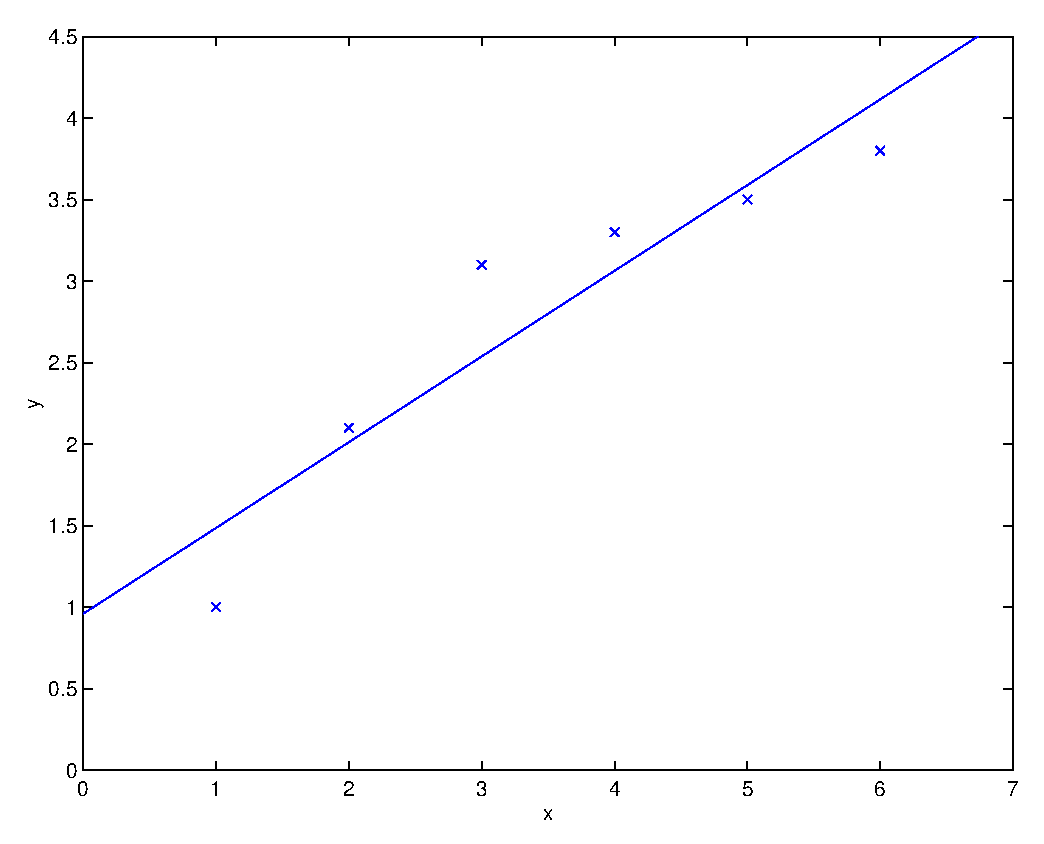
\includegraphics[width=.3\textwidth]{regressionPoly1.eps}\hfill
  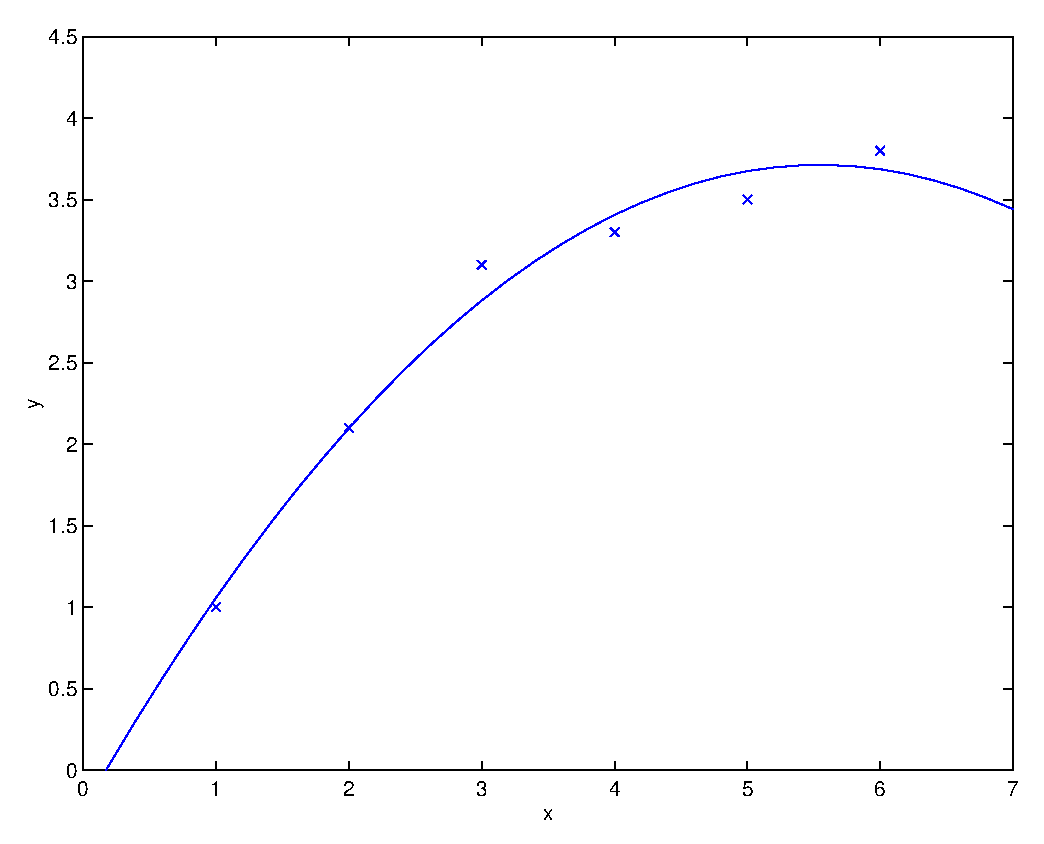
\includegraphics[width=.3\textwidth]{regressionPoly2.eps}\hfill
  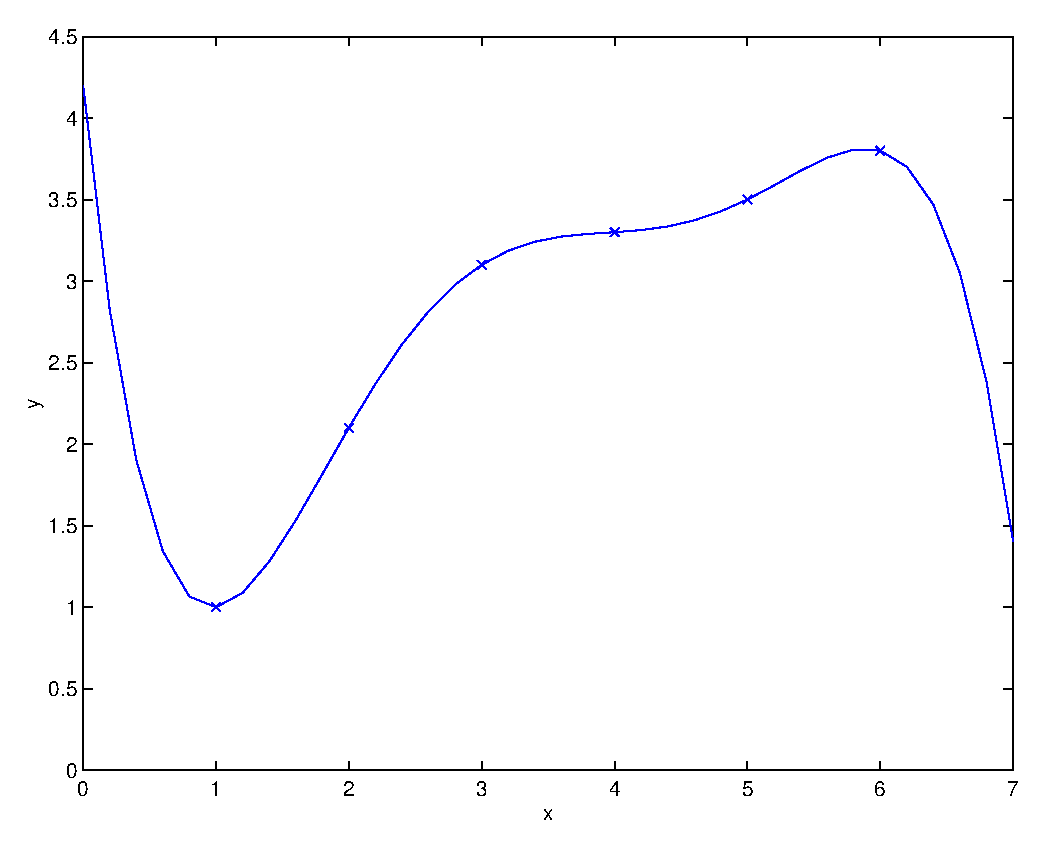
\includegraphics[width=.3\textwidth]{regressionPoly5.eps}
\end{center}

Instead, if we had added an extra feature $x^2$, and fit
$y = \theta_0 + \theta_1 x + \theta_2 x^2$, then we obtain a slightly better
fit to the data.  (See middle figure)  Naively, it might seem that the more
features we add, the better.  However, there is also a danger in adding too
many features: The rightmost figure is the result of fitting a 5-th order polynomial
$y = \sum_{j=0}^{5} \theta_j x^j$.  We see that even though the fitted curve
passes through the data perfectly, we would not expect this to be a very good
predictor of, say, housing prices ($y$) for different living areas ($x$).
Without formally defining what these terms mean,
% or stating why the figures on the left and right really do not represent good models,
we'll say the figure on the left shows an instance of
{\bf underfitting}---in which the data clearly shows structure not captured
by the model---and the figure on the right is an example of {\bf overfitting}.
(Later in this class, when we talk about learning theory we'll formalize
some of these notions, and also define more carefully just what it means for
a hypothesis to be good or bad.)

As discussed previously, and as shown in the example above, the choice
of features is important to ensuring good performance of a learning algorithm.
(When we talk about model selection, we'll also see algorithms for automatically
choosing a good set of features.)  In this section, let us talk
briefly talk about the locally weighted linear regression (LWR) algorithm which,
assuming there is sufficient training data, makes the choice of features
less critical.  This treatment will be brief, since you'll get a chance to
explore some of the properties of the LWR algorithm yourself in the homework.

In the original linear regression algorithm, to make a prediction at a query
point $x$ (i.e., to evaluate $h(x)$), we would:
\begin{enumerate}
\item Fit $\theta$ to minimize $\sum_i (\ysi - \theta^T\xsi)^2$.
\item Output $\theta^Tx$.
\end{enumerate}

In contrast, the locally weighted linear regression algorithm does the following:
\begin{enumerate}
\item Fit $\theta$ to minimize $\sum_i \wsi (\ysi - \theta^T\xsi)^2$.
\item Output $\theta^Tx$.
\end{enumerate}
Here, the $\wsi$'s are non-negative valued {\bf weights}. Intuitively, if $\wsi$
is large for a particular value of $i$, then in picking $\theta$, we'll try hard to
make $(\ysi - \theta^T\xsi)^2$ small.  If $\wsi$ is small, then the
$(\ysi - \theta^T\xsi)^2$ error term will be pretty much ignored in the fit.

A fairly standard choice for the weights is\footnote{If $x$ is vector-valued,
this is generalized to be
$\wsi = \exp(-(\xsi - x)^T(\xsi-x)/(2\tau^2))$, or
$\wsi = \exp(-(\xsi - x)^T\Sigma^{-1}(\xsi-x)/2)$, for
an appropriate choice of $\tau$ or $\Sigma$.}
\[
\wsi = \exp\left(-\frac{(\xsi - x)^2}{2\tau^2}\right)
\]
Note that the weights depend on the particular point $x$ at which we're
trying to evaluate $x$.  Moreover, if $|\xsi - x|$ is small, then $\wsi$ is
close to 1; and if $|\xsi-x|$ is large, then $\wsi$ is small.  Hence, $\theta$
is chosen giving a much higher ``weight'' to the (errors on) training
examples close to the query point $x$.  (Note also that while the formula
for the weights takes a form that is cosmetically similar to the
density of a Gaussian distribution, the $\wsi$'s do not directly have
anything to do with Gaussians, and in particular the $\wsi$ are not random
variables, normally distributed or otherwise.)
The parameter $\tau$ controls how quickly the weight of a training example
falls off with distance of its $\xsi$ from the query point $x$; $\tau$ is called
the {\bf bandwidth} parameter, and is also something that you'll get to
experiment with in your homework.

Locally weighted linear regression is the first example we're seeing
of a {\bf non-parametric} algorithm.  The (unweighted) linear regression
algorithm that we saw earlier is known as a {\bf parametric} learning
algorithm, because it has a fixed, finite number of parameters
(the $\theta_i$'s), which are
fit to the data.  Once we've fit the $\theta_i$'s and stored them away, we no
longer need to keep the training data around to make future predictions.
In contrast, to make predictions using locally weighted linear regression,
we need to keep the entire training set around.  The term ``non-parametric''
(roughly) refers to the fact that the amount of stuff we need to keep
%(the number of ``parameters'')
in order to represent the hypothesis $h$
grows linearly with the size of the training set.

%\newpage
\part{Classification and logistic regression}

Let's now talk about the classification problem.  This is just like
the regression problem, except that the values $y$ we now want to
predict take on only a small number of discrete values.  For now,
we will focus on the {\bf binary classification} problem in
which $y$ can take on only two values, 0 and 1.
(Most of what we
say here will also generalize to the multiple-class case.)
For instance, if we are trying to build a spam classifier for email,
then $\xsi$ may be some features of a piece of email, and $y$ may
be 1 if it is a piece of spam mail, and 0 otherwise.
0 is also called the {\bf negative class}, and
1 the {\bf positive class}, and they are sometimes also denoted
by the symbols ``-'' and ``+.'' Given $\xsi$, the corresponding
$\ysi$ is also called the {\bf label} for the training example.

\section{Logistic regression}

We could approach the classification problem ignoring the fact that
$y$ is discrete-valued, and use our old linear regression algorithm to
try to predict $y$ given $x$. However, it is easy to construct examples
where this method performs very poorly.
\iffalse
One standard example
is as follows: Suppose we are using stochastic gradient descent,
and encounter a training example on which $h_\theta(x) = 100$, and
where $y = 1$.  Since $h_\theta(x) \gg 1$, the only reasonable interpretation
of the predicted value of $y$ on this example is that it is probably
$1$; so, we actually classified it correctly. However, in the LMS
update rule, $\theta_j := \theta_j + \alpha \left(\ysi - h_\theta(\xsi)\right) \xsi_j$,
the error term $y - h_\theta(\xsi)$ will be huge, and we may end up making
a huge change to our weights for this example that we've essentially
classified correctly, quite likely at the cost of worsening our prediction
on some other examples.
\fi
Intuitively, it also doesn't make sense for $h_\theta(x)$ to take
values larger than 1 or smaller than 0 when we know that $y \in \{0,1\}$.

To fix this, let's change the form for our hypotheses $h_\theta(x)$.  We
will choose
\[
h_\theta(x) = g(\theta^Tx) = \frac{1}{1+e^{-\theta^Tx}},
\]
where
\[
g(z) = \frac{1}{1+e^{-z}}
\]
is called the {\bf logistic function} or the {\bf sigmoid function}.
Here is a plot showing $g(z)$:
\begin{center}
% Commenting out since outdated class eps to integrate images
% \epsfxsize=3in
% \epsffile{sigmoid.eps}
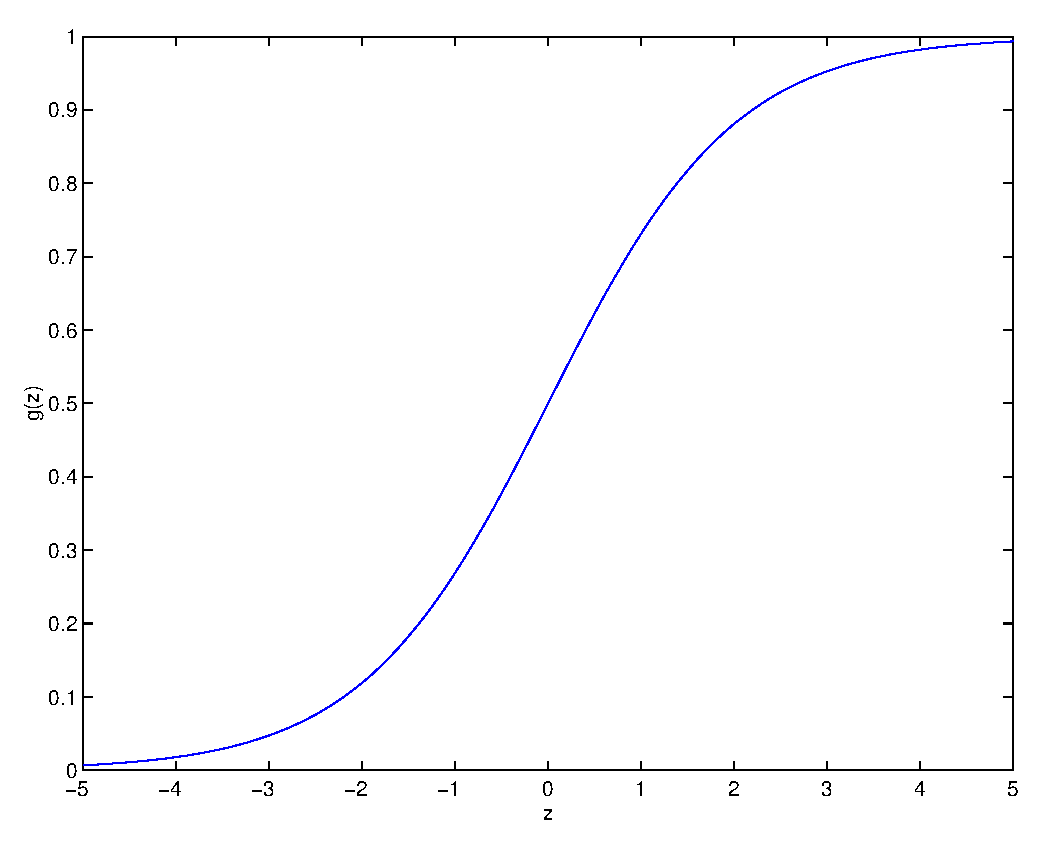
\includegraphics[scale=0.4]{sigmoid.eps}
\end{center}
Notice that $g(z)$ tends towards 1 as $z \rightarrow \infty$, and $g(z)$ tends
towards 0 as $z \rightarrow -\infty$.  Moreover, g(z), and hence also $h(x)$, is
always bounded between 0 and 1.  As before, we are keeping the convention
of letting $x_0=1$, so
that $\theta^Tx = \theta_0 + \sum_{j=1}^\di \theta_j x_j$.

For now, let's take the choice of $g$ as given.  Other functions that smoothly
increase from 0 to 1 can also be used, but for a couple of reasons that we'll
see later (when we talk about GLMs, and when we talk about generative
learning algorithms),
the choice of the logistic function is a fairly natural one.
Before moving on, here's a useful property of the derivative of the sigmoid function,
which we write as $g'$:
\begin{eqnarray*}
g'(z) &=& \frac{d}{dz} \;\frac{1}{1+e^{-z}} \\
&=&\frac{1}{(1+e^{-z})^2}\left(e^{-z}\right) \\
&=& \frac{1}{(1+e^{-z})}\cdot \left(1 - \frac{1}{(1+e^{-z})}\right) \\
&=& g(z) (1-g(z)).
\end{eqnarray*}

So, given the logistic regression model, how do we fit $\theta$ for it?  Following how
we saw least squares regression could be derived as the maximum likelihood estimator
under a set of assumptions,
let's endow our classification model with a set of probabilistic assumptions,
and then fit the parameters via maximum likelihood.

Let us assume that
\begin{eqnarray*}
P(y=1 \mid x; \theta) &=& h_\theta(x) \\
P(y=0 \mid x; \theta) &=& 1- h_\theta(x) \\
\end{eqnarray*}
Note that this can be written more compactly as
\begin{eqnarray*}
p(y \mid x; \theta) = \left(h_\theta(x)\right)^y \left(1-h_\theta(x)\right)^{1-y}
\end{eqnarray*}
Assuming that the $\nexp$ training examples were generated independently, we can then
write down the likelihood of the parameters as
\begin{eqnarray*}
L(\theta) &=& p(\vecy \mid X ; \theta) \\
&=& \prod_{i=1}^\nexp p(\ysi\mid \xsi;\theta) \\
&=& \prod_{i=1}^\nexp \left(h_\theta(\xsi)\right)^\ysi \left(1-h_\theta(\xsi)\right)^{1-\ysi}
\end{eqnarray*}
As before, it will be easier to maximize the log likelihood:
\begin{eqnarray*}
\ell(\theta) &=& \log L(\theta) \\
&=& \sum_{i=1}^\nexp \ysi \log h(\xsi) + (1-\ysi) \log(1- h(\xsi))
\end{eqnarray*}

How do we maximize the likelihood?  Similar to our derivation in the case
of linear regression, we can use gradient ascent.  Written in vectorial
notation, our updates will therefore be given by
$\theta := \theta + \alpha \nabla_\theta \ell(\theta)$.  (Note the
positive rather than negative sign in the update formula, since we're maximizing, rather
than minimizing, a function now.)  Let's start by working with just
one training example $(x,y)$, and take derivatives to derive the stochastic
gradient ascent rule:
\begin{eqnarray*}
\frac{\partial}{\partial \theta_j} \ell(\theta) &=&
\left(y \frac{1}{g(\theta^Tx)} - (1-y) \frac{1}{1-g(\theta^Tx)}\right)
\frac{\partial}{\partial \theta_j} g(\theta^Tx) \\
&=& \left(y \frac{1}{g(\theta^Tx)} - (1-y) \frac{1}{1-g(\theta^Tx)}\right)
g(\theta^Tx)(1-g(\theta^Tx))
\frac{\partial}{\partial \theta_j} \theta^Tx \\
&=& \left(y (1-g(\theta^Tx)) - (1-y) g(\theta^Tx) \right) x_j \\
&=& \left(y - h_\theta(x) \right) x_j
\end{eqnarray*}
Above, we used the fact that $g'(z) = g(z)(1-g(z))$. This therefore gives
us the stochastic gradient ascent rule
\[
\theta_j := \theta_j + \alpha \left(\ysi - h_\theta(\xsi)\right) x^{(i)}_j
\]
If we compare this to the LMS update rule, we see that it looks identical;
but this is \emph{not} the same algorithm, because $h_\theta(\xsi)$ is now
defined as a non-linear function of $\theta^T\xsi$.  Nonetheless, it's a little
surprising that we end up with the same update rule for a rather different
algorithm and learning problem.  Is this coincidence, or is there a deeper
reason behind this?  We'll answer this when we get to GLM models.  (See also
the extra credit problem on Q3 of problem set 1.)

\section{Digression: The perceptron learning algorithm}

We now digress to talk briefly about an algorithm that's
of some historical interest, and that we will also return to later when
we talk about learning theory.  Consider
modifying the logistic regression method to ``force'' it to output values
that are either 0 or 1 or exactly.  To do so, it seems natural to change the definition
of $g$ to be the threshold function:
\[
 g(z) = \left\{\begin{array}{ll}
 1  & \mbox{if~} z \geq 0 \\
 0  & \mbox{if~} z < 0
\end{array} \right.
\]
If we then let $h_\theta(x) = g(\theta^Tx)$ as before but using this
modified definition of $g$, and if we use the update rule
\[
\theta_j := \theta_j + \alpha \left(\ysi - h_\theta(\xsi)\right) x^{(i)}_j.
\]
then we have the {\bf perceptron learning algorithm}.

In the 1960s, this ``perceptron'' was argued to be a rough model for
how individual neurons in the brain work.  Given how simple the algorithm
is, it will also provide a starting point for our analysis when we talk
about learning theory later in this class.  Note however
that even though the perceptron may be cosmetically similar to the other
algorithms we talked about, it is actually a very different type of algorithm
than logistic regression and least squares linear regression;
in particular, it is difficult to endow the perceptron's predictions
with meaningful probabilistic interpretations, or derive the perceptron
as a maximum likelihood estimation algorithm.

\section{Another algorithm for maximizing $\ell(\theta)$}

Returning to logistic regression with $g(z)$ being the sigmoid function,
let's now talk about a different algorithm for maximizing $\ell(\theta)$.

To get us started, let's consider Newton's method for finding a zero
of a function.  Specifically,
suppose we have some function $f : \Re \mapsto \Re$, and we wish to
find a value of $\theta$ so that $f(\theta) = 0$.
Here, $\theta \in \Re$ is a real number.  Newton's method performs the following
update:
\[
\theta := \theta - \frac{f(\theta)}{f'(\theta)}.
\]
This method has a natural interpretation in which we can think of it as
approximating the function $f$ via a linear function that is tangent to
$f$ at the current guess $\theta$, solving for where that linear function
equals to zero, and letting the next guess for $\theta$ be where that linear
function is zero.

Here's a picture of the Newton's method in action:

% Function within macros.tex irrevalent since using eps library
% \threefigboxnolabel{newton1.eps}{newton2.eps}{newton3.eps}
\begin{center}
  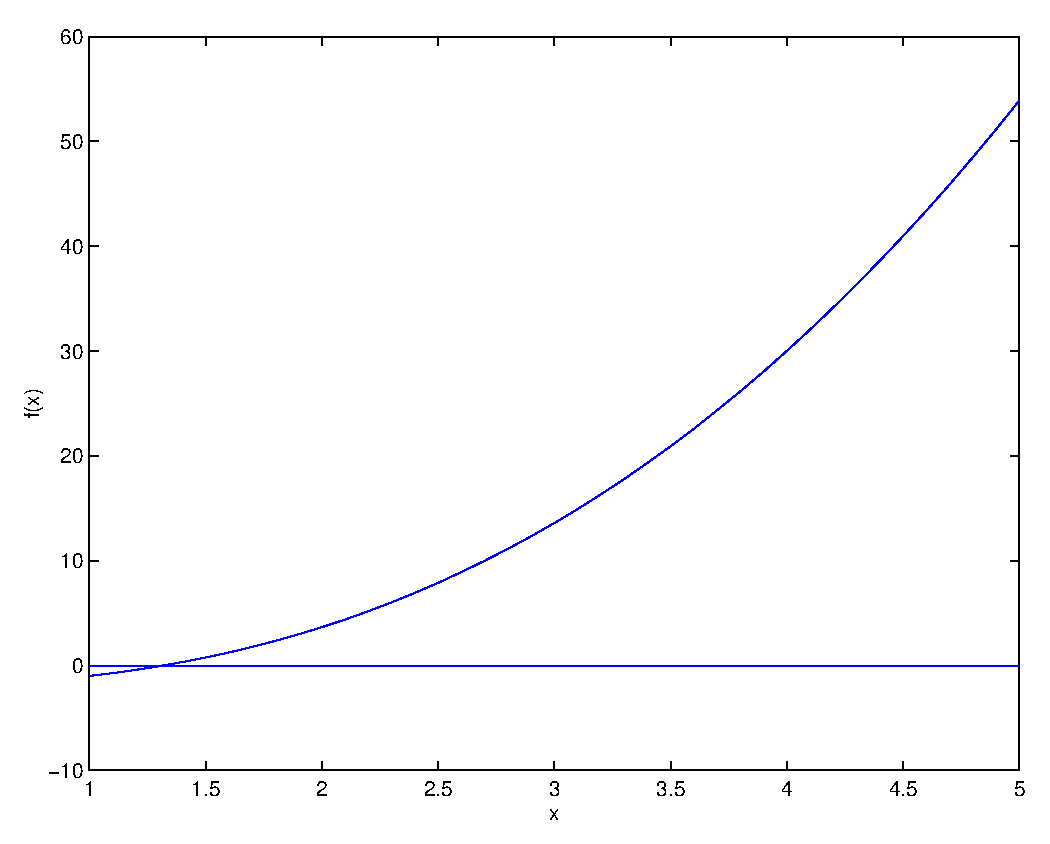
\includegraphics[width=.3\textwidth]{newton1.eps}\hfill
  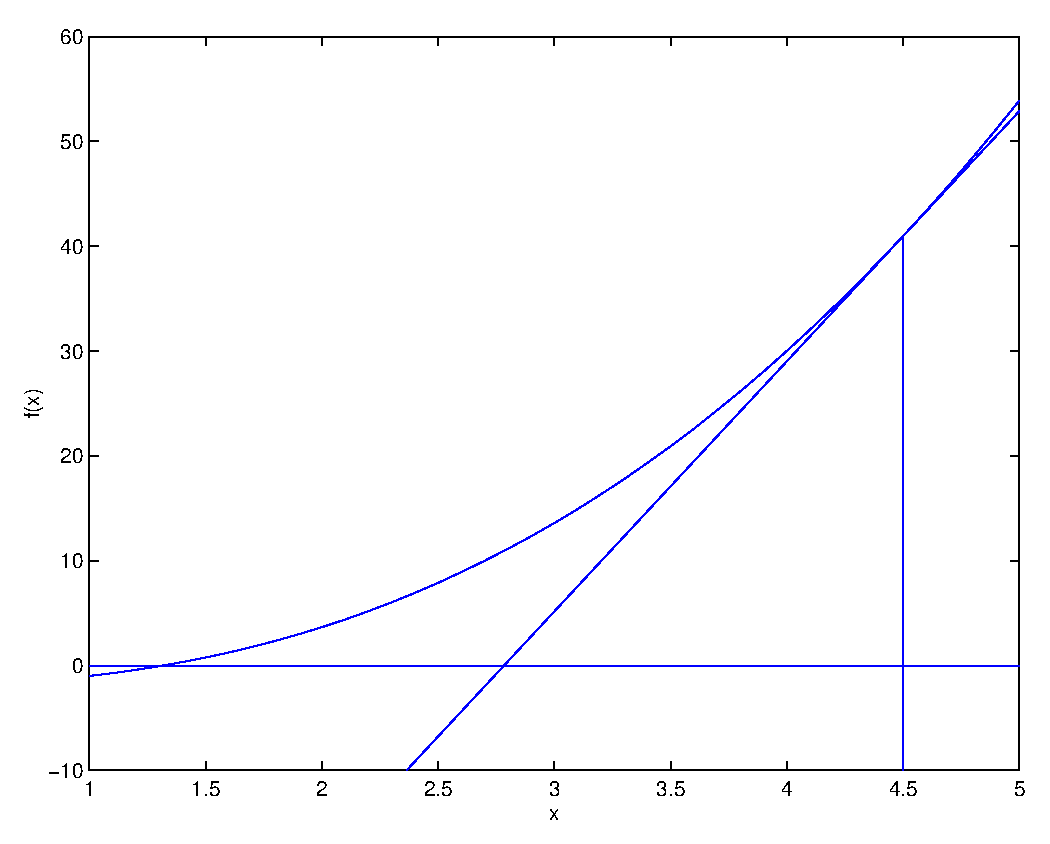
\includegraphics[width=.3\textwidth]{newton2.eps}\hfill
  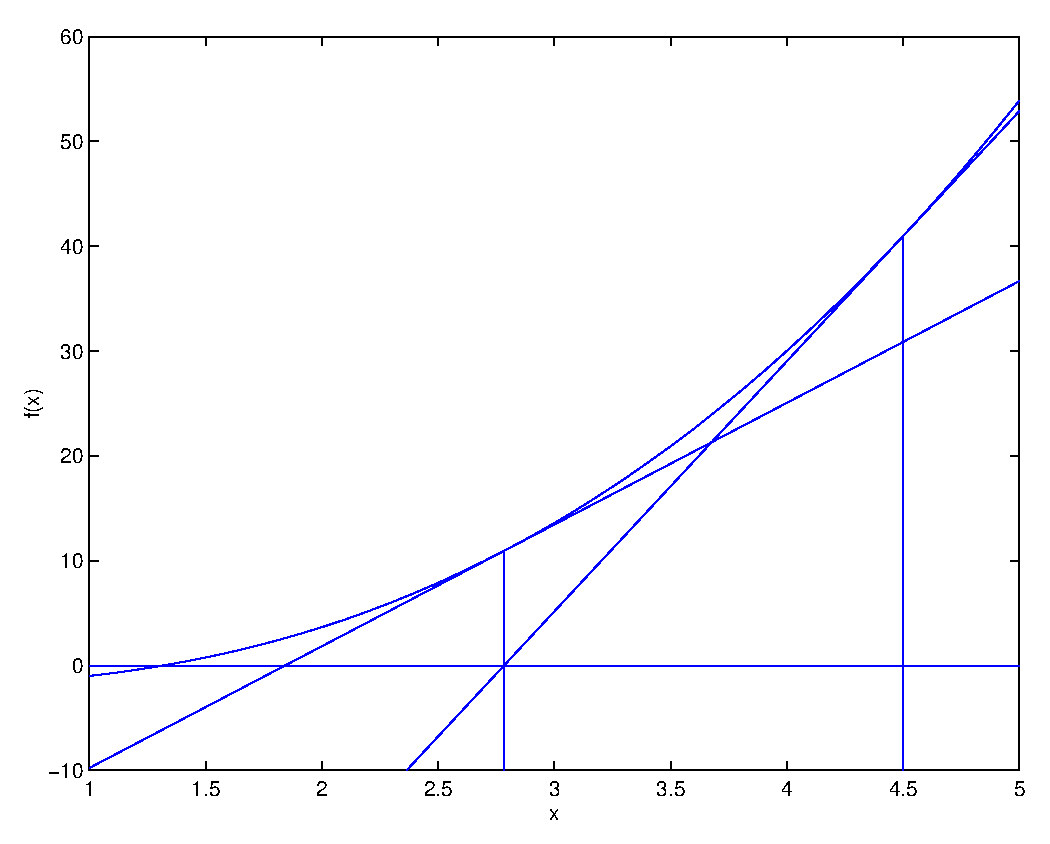
\includegraphics[width=.3\textwidth]{newton3.eps}
\end{center}

In the leftmost figure, we see the function $f$ plotted along with the
line $y=0$.  We're trying to find $\theta$ so that $f(\theta)=0$; the value
of $\theta$ that achieves this is about 1.3.
Suppose we initialized the algorithm with $\theta=4.5$.  Newton's method
then fits a straight line tangent to $f$ at $\theta=4.5$, and solves for
the where that line evaluates to 0.  (Middle figure.)  This give us the
next guess for $\theta$, which is about 2.8.  The rightmost figure shows the result
of running one more iteration, which the updates $\theta$ to about 1.8.
After a few more iterations, we rapidly approach $\theta = 1.3$.

Newton's method gives a way of getting to $f(\theta)=0$.  What if we want
to use it to maximize some function $\ell$?  The maxima of $\ell$ correspond
to points where its first derivative $\ell'(\theta)$ is zero.  So, by letting
$f(\theta) = \ell'(\theta)$, we can use the same algorithm to maximize $\ell$,
and we obtain update rule:
\[
\theta := \theta - \frac{\ell'(\theta)}{\ell''(\theta)}.
\]
(Something to think about: How would this change if we wanted to
use Newton's method to minimize rather than maximize a function?)

%Specifically, it converges quadratically, whereas
%gradient descent converges only linearly.  What this roughly means is that
%if $\epsilon_t$ is, say, $|\theta-\theta^\ast|$, where

Lastly, in our logistic regression setting, $\theta$ is vector-valued, so
we need to generalize Newton's method to this setting.  The generalization of
Newton's method to this multidimensional setting (also called the
Newton-Raphson method) is given by
\[
\theta := \theta - H^{-1} \nabla_\theta \ell(\theta).
\]
Here, $\nabla_\theta \ell(\theta)$ is, as usual, the vector of partial derivatives
of $\ell(\theta)$ with respect to the $\theta_i$'s; and $H$ is an $\di$-by-$\di$
matrix (actually, $\di$+1$-by-$\di$+1$, assuming that we include the intercept term)
called the {\bf Hessian}, whose entries are given by
\[
H_{ij} = \frac{\partial^2 \ell(\theta)}{\partial \theta_i \partial \theta_j}.
\]

Newton's method typically enjoys faster convergence than (batch) gradient
descent, and requires many fewer iterations to get very close to the
minimum.  One iteration of Newton's can, however, be more expensive than one
iteration of gradient descent, since it requires finding and
inverting an $\di$-by-$\di$ Hessian; but so long as $\di$ is not too large,
it is usually much faster overall.  When Newton's method is applied to maximize the
logistic regression log likelihood function $\ell(\theta)$, the resulting method
is also called {\bf Fisher scoring}.
%is also called (a special case of) {\bf Fisher scoring}.

\newpage
\part{Generalized Linear
  Models\hbox to 0.008in{}\protect\LARGE\protect\footnote{The presentation of the
material in this section takes inspiration from Michael I. Jordan, \emph{Learning
in graphical models} (unpublished book draft), and also McCullagh and Nelder,
\emph{Generalized Linear Models (2nd ed.)}.}
}

So far, we've seen a regression example, and a classification example.
In the regression example, we had $y|x;\theta \sim \calN(\mu, \sigma^2)$, and
in the classification one, $y|x;\theta \sim \Ber(\phi)$,
for some appropriate definitions of $\mu$ and $\phi$
%(the means of the normal and of the Bernoulli distributions respectively)
as functions
of $x$ and $\theta$.  In this section, we will show that both of
these methods are special cases of  a broader family of models, called
Generalized Linear Models (GLMs).  We will also show how other models
in the GLM family can be derived and applied to other classification
and regression problems.
%\footnote{The
%presentation of the material on GLMs is based primarily on Jordan, Learning
%in graphical models (unpublished book draft), and also on McCullagh and Nelder,
%Generalized Linear Models (2nd ed.).}

\section{The exponential family}

To work our way up to GLMs, we will begin by defining exponential family distributions.
We say that a class of distributions is in the exponential family if it can be written
in the form
\begin{equation}
p(y;\eta) = b(y) \exp(\eta^T T(y) - a(\eta))        \label{eqn-expfamily}
\end{equation}
Here, $\eta$ is called the {\bf natural parameter}
(also called the {\bf canonical parameter}) of the distribution;
$T(y)$ is the {\bf sufficient statistic} (for the distributions we consider,
it will often be the case that $T(y)=y$); and $a(\eta)$ is the {\bf log partition
function}.  The quantity $e^{-a(\eta)}$ essentially plays the role of a normalization
constant, that makes sure the distribution $p(y;\eta)$ sums/integrates over $y$ to 1.

A fixed choice of $T$, $a$ and $b$ defines a \emph{family} (or set) of distributions
that is parameterized by $\eta$; as we vary $\eta$, we then get different distributions
within this family.

We now show that the Bernoulli and the Gaussian distributions are examples of exponential family distributions.
The Bernoulli distribution with mean $\phi$,
written $\Ber(\phi)$, specifies a distribution over $y \in \{0,1\}$, so that
$p(y=1;\phi)=\phi$; $p(y=0;\phi)=1-\phi$.  As we vary $\phi$, we obtain Bernoulli
distributions with different means.  We now show that this class of Bernoulli
distributions, ones obtained by varying $\phi$, is in the exponential family; i.e.,
that there is a choice of $T$, $a$ and $b$ so that Equation~(\ref{eqn-expfamily})
becomes exactly the class of Bernoulli distributions.

We write the Bernoulli distribution as:
\begin{eqnarray*}
p(y;\phi) &=& \phi^y (1-\phi)^{1-y} \\
&=& \exp(y\log\phi + (1-y) \log(1-\phi)) \\
&=& \exp\left( \left(\log\left(\frac{\phi}{1-\phi}\right)\right)y + \log(1-\phi)\right).
\end{eqnarray*}
Thus, the natural parameter is given by $\eta = \log(\phi/(1-\phi))$.
Interestingly, if we invert this definition for $\eta$ by solving
for $\phi$ in terms of $\eta$, we obtain $\phi = 1/(1+e^{-\eta})$.  This is
the familiar sigmoid function!  This will come up again when we derive logistic
regression as a GLM.  To complete the formulation of the Bernoulli
distribution as an exponential family
distribution, we also have
\begin{eqnarray*}
T(y) &=& y \\
a(\eta) &=& -\log(1-\phi) \\
  &=& \log(1+e^\eta) \\
b(y)&=&1
\end{eqnarray*}
This shows that the Bernoulli distribution can be written in the form
of Equation~(\ref{eqn-expfamily}), using an appropriate choice of $T$, $a$ and $b$.

Let's now move on to consider the Gaussian distribution.  Recall that, when deriving
linear regression, the value of $\sigma^2$ had no effect on our final choice of $\theta$
and $h_\theta(x)$.  Thus, we can choose an arbitrary value for $\sigma^2$ without
changing anything. To simplify the derivation below, let's
set $\sigma^2=1$.\footnote{If we leave $\sigma^2$ as a variable, the Gaussian
distribution can also be shown to be in the exponential family, where $\eta \in \Re^2$
is now a 2-dimension vector that depends on both $\mu$ and $\sigma$.  For the purposes
of GLMs, however, the $\sigma^2$ parameter can also be treated by considering
a more general definition of the exponential family:
$p(y;\eta,\tau) = b(a,\tau) \exp((\eta^T T(y) - a(\eta))/c(\tau))$.
Here, $\tau$ is called the {\bf dispersion parameter}, and for the Gaussian,
$c(\tau) = \sigma^2$; but given our simplification above, we won't need
the more general definition for the examples we will consider here.}
We then have:
\begin{eqnarray*}
p(y;\mu) &=& \frac{1}{\sqrt{2\pi}} \exp\left(-\frac{1}{2} (y-\mu)^2\right) \\
%&=& \frac{1}{\sqrt{2\pi}} \exp\left(-\frac{1}{2} y^2 + \mu y - \frac{1}{2}\mu^2\right)\\
&=& \frac{1}{\sqrt{2\pi}} \exp\left(-\frac{1}{2} y^2 \right) \cdot \exp\left(\mu y - \frac{1}{2}\mu^2\right)
\end{eqnarray*}
Thus, we see that the Gaussian is in the exponential family, with
\begin{eqnarray*}
\eta &=& \mu \\
T(y)&=&y\\
a(\eta) &=& \mu^2/2 \\
  &=& \eta^2/2\\
b(y) &=& (1/\sqrt{2\pi})\exp(-y^2/2).
\end{eqnarray*}

There're many other distributions that are members of the exponential family:
The multinomial (which we'll see later), the Poisson (for modelling count-data;
also see the problem set); the gamma and the exponential (for modelling continuous,
non-negative random variables, such as time-intervals); the beta and the Dirichlet
(for distributions over probabilities); and many more.  In the next section, we
will describe a general ``recipe'' for constructing models in which $y$
(given $x$ and $\theta$) comes from any of these distributions.

\section{Constructing GLMs}

Suppose you would like to build a model to estimate the number $y$ of customers
arriving in your store (or number of page-views on your website) in any given
hour, based on certain features $x$ such as store promotions, recent
advertising, weather, day-of-week, etc.  We know that the Poisson distribution
usually gives a good model for numbers of visitors.
%So, conditioned on the
%features $x$, we might model $y$ as distributed according to a Poisson
%distribution (that has some mean that depends in some way on $x$).
Knowing this, how can we come up with a model for our problem?  Fortunately,
the Poisson is an exponential family distribution, so we can apply a Generalized
Linear Model (GLM).
%so, we will
%be able to derive a GLM for this problem.
In this section, we will we will describe a method for
constructing GLM models for problems such as these.

More generally, consider a classification or regression problem where we would
like to predict the value of some random variable $y$ as a function of $x$.
To derive a GLM for this problem, we will make the following three
assumptions about the conditional distribution of $y$ given $x$ and
about our model:
\begin{enumerate}
\item $y\mid x; \theta \sim {\rm ExponentialFamily}(\eta)$.  I.e.,
given $x$ and $\theta$, the distribution of $y$ follows some
exponential family distribution, with parameter $\eta$.
\item Given $x$, our goal is to predict the expected value of $T(y)$ given $x$.
In most of our examples, we will have $T(y)=y$, so this means we would like
the prediction $h(x)$ output by our learned hypothesis $h$ to
satisfy $h(x) = \E[y|x]$.
(Note that this assumption is satisfied in the choices for $h_\theta(x)$ for
both logistic regression and linear regression.
%, under the probabilistic interpretations of both models.
For instance, in logistic regression,
we had $h_\theta(x) = p(y=1 | x;\theta) =
0 \cdot p(y=0 | x;\theta)
+ 1 \cdot p(y=1 | x;\theta) =
\E[y|x;\theta]$.)
\item The natural parameter $\eta$ and the inputs $x$ are related
linearly: $\eta = \theta^Tx$.
(Or, if $\eta$ is vector-valued, then $\eta_i = \theta_i^Tx$.)
\end{enumerate}

The third of these assumptions might seem the least well justified of the
above, and it might be better thought of as a ``design choice'' in our
recipe for designing GLMs, rather than as an assumption per se.  These
three assumptions/design choices will allow us to derive a
very elegant class
of learning algorithms, namely GLMs, that have many desirable
properties such as ease of learning.
%there being no local optima in the log-likelihood,
%making parameter learning relatively easy.
Furthermore, the resulting
models are often very effective for modelling different types of
distributions over $y$; for example, we will shortly show that
both logistic regression and ordinary least squares
%(perhaps the two most widely used learning algorithms in the world)
can both be
derived as GLMs.


\subsection{Ordinary Least Squares}

To show that ordinary least squares is a special case of the GLM family of
models, consider the setting where the target variable $y$ (also called the {\bf response variable}
in GLM terminology) is continuous, and we model the conditional
distribution of $y$ given $x$ as a Gaussian $\calN(\mu,\sigma^2)$.
(Here, $\mu$ may depend $x$.)  So, we let the $ExponentialFamily(\eta)$
distribution above be the Gaussian distribution.  As we saw previously, in
the formulation of the Gaussian as an exponential family distribution, we had
$\mu = \eta$.  So, we have
\begin{eqnarray*}
h_\theta(x) &=& E[y|x;\theta] \\
&=& \mu \\
&=& \eta \\
&=& \theta^Tx.
\end{eqnarray*}
The first equality follows from Assumption 2, above; the second equality follows
from the fact that $y | x;\theta \sim \calN(\mu,\sigma^2)$, and so its expected
value is given by $\mu$; the third equality follows from Assumption 1 (and our earlier
derivation showing that $\mu=\eta$ in the formulation of the Gaussian as
an exponential family distribution); and the
last equality follows from Assumption 3.

\subsection{Logistic Regression}

We now consider logistic regression.  Here we are interested in binary
classification, so $y \in \{0,1\}$.  Given that $y$ is binary-valued, it therefore seems natural to choose
the Bernoulli family of distributions to model the conditional distribution of
$y$ given $x$.  In our formulation of the Bernoulli distribution as an exponential
family distribution, we had $\phi = 1/(1+e^{-\eta})$.  Furthermore, note
that if $y|x;\theta \sim \Ber(\phi)$, then
$\E[y|x;\theta] = \phi$.  So, following a similar derivation as the one for
ordinary least squares, we get:
\begin{eqnarray*}
h_\theta(x) &=& E[y|x;\theta] \\
&=& \phi \\
&=& 1/(1+e^{-\eta}) \\
&=& 1/(1+e^{-\theta^Tx})
\end{eqnarray*}
So, this gives us hypothesis functions of the form $h_\theta(x) = 1/(1+e^{-\theta^Tx})$.
If you are previously wondering how we came up with the form of the
logistic function $1/(1+e^{-z})$, this gives one answer:  Once we
assume that $y$ conditioned on $x$ is Bernoulli, it arises as
a consequence of the definition of GLMs and exponential family distributions.

To introduce a little more terminology, the function $g$ giving the distribution's mean as
a function of the natural parameter ($g(\eta) = \E[T(y);\eta]$) is called
the {\bf canonical response function}.  Its inverse, $g^{-1}$, is called
the {\bf canonical link function}.  Thus, the canonical response function
for the Gaussian family is just the identify function; and the canonical
response function for the Bernoulli is the logistic function.\footnote{Many
texts use $g$ to denote the link function, and $g^{-1}$ to denote the response
function; but the notation we're using here, inherited from the early machine
learning literature, will be more consistent with the notation used in the
rest of the class.}

\subsection{Softmax Regression}

Let's look at one more example of a GLM.  Consider a classification problem in which
the response variable $y$ can take on any one of $k$ values,
so $y \in \{1, 2, \ldots, k\}$.  For example, rather than classifying email into
the two classes spam or not-spam---which would have been a binary
classification problem---we might want to classify it into three classes,
such as spam, personal mail, and work-related mail.  The response variable is
still discrete, but can now take on more than two values.  We will
thus model it as distributed according to a multinomial distribution.

Let's derive a GLM for modelling this type of multinomial data.  To do so, we will
begin by expressing the multinomial as an exponential family distribution.

To parameterize a multinomial over $k$ possible outcomes, one could use $k$ parameters
$\phi_1, \ldots, \phi_k$ specifying the probability of each of the outcomes.  However,
these parameters would be redundant, or more formally, they would not be
independent (since knowing any $k-1$ of the $\phi_i$'s uniquely determines
the last one, as they must satisfy $\sum_{i=1}^k \phi_i$ = 1).  So, we will
instead parameterize the multinomial with only $k-1$ parameters,
$\phi_1, \ldots, \phi_{k-1}$, where $\phi_i = p(y=i;\phi)$, and
$p(y=k;\phi)=1-\sum_{i=1}^{k-1} \phi_i$.  For notational convenience, we
will also let $\phi_k = 1-\sum_{i=1}^{k-1} \phi_i$, but we should keep in mind that this
is not a parameter, and that it is fully specified by $\phi_1, \ldots, \phi_{k-1}$.

%To parameterize a multinomial over $k$ possible outcomes, we need $k-1$ parameters.
%Our parameters will be
%$\phi_1, \ldots, \phi_{k-1}$, where $\phi_i = p(y=i;\phi)$,
%and $p(y=k)=1-\sum_{i=1}^{k-1} \phi_i$.  For notational convenience, we
%will also let $\phi_k = 1-\sum_{i=1}^{k-1} \phi_i$, but we should keep
%in mind that $\phi_k$ isn't really itself a parameter, and that it is fully specified
%by the parameters $\phi_1, \ldots, \phi_{k-1}$.

To express the multinomial as an exponential family distribution, we will define
$T(y) \in \Re^{k-1}$ as follows:
{\footnotesize
\[
T(1) = \left[ \begin{tabular}{c} 1 \\ 0 \\ 0 \\ \vdots \\ 0 \end{tabular}\right], \;
T(2) = \left[ \begin{tabular}{c} 0 \\ 1 \\ 0 \\ \vdots \\ 0 \end{tabular}\right], \;
T(3) = \left[ \begin{tabular}{c} 0 \\ 0 \\ 1 \\ \vdots \\ 0 \end{tabular}\right], \;
\cdots,
T(k-1) = \left[ \begin{tabular}{c} 0 \\ 0 \\ 0 \\ \vdots \\ 1 \end{tabular}\right], \;
T(k) = \left[ \begin{tabular}{c} 0 \\ 0 \\ 0 \\ \vdots \\ 0 \end{tabular}\right], \;
\]
}%
Unlike our previous examples, here we do \emph{not} have $T(y) = y$; also,
$T(y)$ is now a $k-1$ dimensional vector, rather than a real number.
We will write $(T(y))_i$ to denote the $i$-th element of the vector $T(y)$.

%For notational
%convenience, we will also use $\ytil$ as a shorthand to denote $T(y)$.

We introduce one more very useful piece of notation.  An indicator function $1\{\cdot\}$
takes on a value of 1 if its argument is true, and 0 otherwise
($1\{{\rm True}\}=1$, $1\{{\rm False}\}=0$).  For example, $1\{2=3\}=0$,
and $1\{3=5-2\}=1$.  So, we can also write the relationship between
$T(y)$ and $y$ as $(T(y))_i = 1\{y=i\}$.  (Before you continue reading,
please make sure you understand why this is true!)  Further, we
have that $\E[(T(y))_i] = P(y=i) = \phi_i$.
%In the sequel, we will switch freely
%between the $y$ and the $(T(y))_i$ notation, with the understanding that
%they are related this way.

%\ytil \in
%We've been thinking of $y$ as taking values in the set $\{1\,2, \ldots, k\}$, but
%``$1,2, \ldots, k$'' are just $k$ arbitrary names for the $k$ classes (such as spam,
%personal mail, work-related mail).  Again for notational convenience, it will
%be useful to instead consider a corresponding random variable $\ytil$,
%taking value as follows:
%\[
%\ytil \in
%\left\{
%\left[ \begin{tabular}{c} 1 \\ 0 \\ 0 \\ \vdots \\ 0 \end{tabular}\right],
%\left[ \begin{tabular}{c} 0 \\ 1 \\ 0 \\ \vdots \\ 0 \end{tabular}\right],
%\cdots,
%\left[ \begin{tabular}{c} 0 \\ 0 \\ 0 \\ \vdots \\ 1 \end{tabular}\right]
%\left[ \begin{tabular}{c} 0 \\ 0 \\ 0 \\ \vdots \\ 0 \end{tabular}\right]
%\right\} \subseteq \Re^{k-1}
%\]

We are now ready to show that the multinomial is a member of the
exponential family. We have:
\begin{eqnarray*}
p(y;\phi)
&=& \phi_1^{1\{y=1\}} \phi_2^{1\{y=2\}} \cdots \phi_k^{1\{y=k\}} \\
&=& \phi_1^{1\{y=1\}} \phi_2^{1\{y=2\}} \cdots \phi_k^{1-\sum_{i=1}^{k-1} 1\{y=i\}} \\
&=& \phi_1^{(T(y))_1} \phi_2^{(T(y))_2} \cdots \phi_k^{1-\sum_{i=1}^{k-1} (T(y))_i} \\
&=& \exp((T(y))_1 \log(\phi_1) +  (T(y))_2 \log(\phi_2) +
    \\
    && \;\;\;\;\;\;\;\;\;
    \cdots +
    \left( {1-{\textstyle \sum_{i=1}^{k-1} (T(y))_i}}\right) \log(\phi_k))\\
&=& \exp((T(y))_1 \log(\phi_1/\phi_k) +  (T(y))_2 \log(\phi_2/\phi_k) +
    \\
    && \;\;\;\;\;\;\;\;\;
    \cdots + (T(y))_{k-1} \log(\phi_{k-1}/\phi_k) + \log(\phi_k))\\
&=& b(y) \exp(\eta^T T(y) - a(\eta))
\end{eqnarray*}
where
\begin{eqnarray*}
\eta &=& \left[ \begin{tabular}{c} $\log (\phi_1/\phi_k)$ \\
$\log (\phi_2/\phi_k)$ \\
$\vdots$ \\
$\log (\phi_{k-1}/\phi_k)$ \end{tabular}  \right], \\
a(\eta) &=& -\log(\phi_k) \\
b(y)&=&1.
\end{eqnarray*}
This completes our formulation of the multinomial as an exponential family
distribution.

The link function is given (for $i=1,\ldots,k$) by
\[
\eta_i = \log \frac{\phi_i}{\phi_k}.
\]
For convenience, we have also defined $\eta_k = \log(\phi_k/\phi_k) = 0$.
To invert the link function and derive the response function, we therefore have
that
\begin{eqnarray}
e^{\eta_i} &=& \frac{\phi_i}{\phi_k}   \nonumber  \\
\phi_k e^{\eta_i} &=& \phi_i    \label{eqn-resp1} \\
\phi_k \sum_{i=1}^k e^{\eta_i} &=& \sum_{i=1}^k \phi_i = 1   \nonumber
\end{eqnarray}
This implies that $\phi_k = 1/\sum_{i=1}^k e^{\eta_i}$, which can be substituted back
into Equation~(\ref{eqn-resp1}) to give the response function
\[
%%E[(T(y))_i | x;\theta] =
\phi_i = \frac{e^{\eta_i}}{\sum_{j=1}^k e^{\eta_j}}
\]
This function mapping from the $\eta$'s to the $\phi$'s is called the
{\bf softmax} function.

To complete our model, we use Assumption 3, given earlier, that
the $\eta_i$'s are linearly related to the $x$'s.  So,
have $\eta_i = \theta_i^T x$ (for $i=1,\ldots, k-1$),
where $\theta_1, \ldots, \theta_{k-1} \in \Re^{\di+1}$ are the parameters of
our model.  For notational convenience, we can also define $\theta_k=0$, so
that $\eta_k=\theta_k^Tx = 0$, as given previously.  Hence, our model assumes
that the conditional distribution of $y$ given $x$ is given by
\begin{eqnarray}
p(y=i|x;\theta)
%&=& E[(T(y))_i | x;\theta]  \\
&=& \phi_i  \nonumber \\
&=& \frac{e^{\eta_i}}{\sum_{j=1}^k e^{\eta_j}} \nonumber \\
&=& \frac{e^{\theta_i^Tx}}{\sum_{j=1}^k e^{\theta_j^Tx}} \label{eqn-softmaxdef}
\end{eqnarray}
This model, which applies to classification problems
where $y \in \{1, \ldots, k\}$, is called {\bf softmax regression}.
It is a generalization of logistic regression.

Our hypothesis will output
\begin{eqnarray*}
h_\theta(x) &=& \E[T(y)|x;\theta] \\
&=& \E \left[ \left. \begin{tabular}{c} $1\{y=1\}$ \\ $1\{y=2\}$ \\ \vdots \\ $1\{y=k-1\}$ \end{tabular} \right|\, x;\theta \right] \\
&=& \left[ \begin{tabular}{c} $\phi_1$ \\ $\phi_2$ \\ \vdots \\ $\phi_{k-1}$ \end{tabular} \right] \\
&=& \left[ \begin{tabular}{c}
$\frac{\exp(\theta_1^Tx)}{\sum_{j=1}^k \exp(\theta_j^Tx)}$ \\
$\frac{\exp(\theta_2^Tx)}{\sum_{j=1}^k \exp(\theta_j^Tx)}$ \\
\vdots \\
$\frac{\exp(\theta_{k-1}^Tx)}{\sum_{j=1}^k \exp(\theta_j^Tx)}$
\end{tabular} \right].
\end{eqnarray*}
In other words, our hypothesis will output the estimated probability that $p(y=i|x;\theta)$, for every
value of $i=1,\ldots,k$.  (Even though $h_\theta(x)$ as defined above is only $k-1$ dimensional,
clearly $p(y=k|x;\theta)$ can be obtained as $1-\sum_{i=1}^{k-1} \phi_i$.)

Lastly, let's discuss parameter fitting. Similar to our original derivation of ordinary least squares
and logistic regression, if we have a training set of $\nexp$ examples $\{(\xsi, \ysi); i=1,\ldots,\nexp\}$
and would like to learn the parameters $\theta_i$ of this model, we would begin by writing
down the log-likelihood
\begin{eqnarray*}
\ell(\theta) &=& \sum_{i=1}^\nexp \log p(\ysi|\xsi;\theta) \\
&=& \sum_{i=1}^\nexp \log \prod_{l=1}^k \left(
    \frac{e^{\theta^T_l\xsi}}{\sum_{j=1}^k e^{\theta^T_j\xsi}} \right)^{1\{\ysi=l\}}
\end{eqnarray*}
To obtain the second line above, we used the definition for $p(y|x;\theta)$ given in Equation~(\ref{eqn-softmaxdef}).
We can now obtain the maximum likelihood estimate of the parameters by maximizing $\ell(\theta)$
in terms of $\theta$, using a method such as gradient ascent or Newton's method.




%\part{Bibliography and end-notes}
%
%The housing prices data used as an example in the discussion of linear regression
%is from a learning and statistics workshop held in Simon Fraser University
%(http://www.stat.sfu.ca/Innovation/WpgMLS/mls.dat).
%This presentation is based on Duda, Hart and Stork, Pattern Classification (2nd ed.);
%Bishop, Neural Networks for Pattern Recognition; and Jordan, Learning in
%Graphical models (unpublished book draft).  The section on GLMs was based on Jordan


%workshop held in Simon Fraser University

\end{document}
